%Tese de Doutorado
%PPGEE - UFMG
%-------------------------------------------------------------------
%Definições gerais do documento
\documentclass[	12pt,				
				openany,			
				oneside,			
				a4paper,
				brazil, % Texts in pt-br
				english ]{book}
%--------------------------------------------------------------------
%Pacotes usados
\usepackage[main=brazil]{babel} % Muda o nome das palavra-chave, como chapter para capítulo
\usepackage[T1]{fontenc}    % Permite copiar textos com acento
\usepackage[utf8]{inputenc} % Permite que eu escreve com acentos pt-br, assim posso digitar à em vez de ter que digitar \'a 
\usepackage{amsmath}
\usepackage[dvips]{graphicx}
\thispagestyle{empty}
\usepackage{times}
\usepackage{epsfig,latexsym}
\usepackage{float}
\usepackage{natbib}
\usepackage{color}
\usepackage{indentfirst}
\usepackage{psfrag}
\usepackage{epsfig}
\usepackage{dsfont}%LUIS muda a fonte
\usepackage{amssymb}%LUIS
\usepackage[mathscr]{euscript}%LUIS alguns simbolos diferentes
\usepackage{accents}%LUIS
%\usepackage{rotating}
\usepackage{fancyhdr}
\usepackage{makeidx}
\usepackage{setspace}
%\usepackage[hang,small]{caption}
\usepackage{ae}
\usepackage{hyperref}
\usepackage{bm}%LUIS
\usepackage[below]{placeins}
\usepackage{flafter}
\usepackage{txfonts} 
\usepackage{pxfonts} % Fonte Book Antiqua
%\usepackage{natbib}
\usepackage{pdfpages}%LUIS Incluir pdf
\usepackage{frcursive}%LUIS possibilita fontes cursivas
\usepackage{amsxtra}%LUIS usado para colocar sptilde ~ no meio do texto
\usepackage{comment}
\usepackage{icomma}%LUIS ajusta as virgulas nas partes numerais
\usepackage{subfigure}
\usepackage[left=2.5cm,right=2.5cm,top=2.5cm,bottom=2.5cm]{geometry}
\usepackage{tabularx}%LUIS
\usepackage{amsmath,amsfonts,amssymb}
\usepackage[table]{xcolor}
\usepackage{multirow}           % Merge rows and columns in tables
\usepackage{longtable}          % Large tables
\usepackage{fancyvrb}           % Codes and Outputs commands
\usepackage{listings}           % Codes and Outputs commands
\usepackage{pdflscape}
\usepackage{float}
\usepackage{latexsym}           % Extra symbols of Latex
\usepackage{booktabs}
\usepackage{enumerate}
\usepackage{acronym}
\usepackage{arydshln}%LUIS linha pontilhada vertical matriz
%\usepackage{algorithm2e}          % Algorithms
%\usepackage[portuguese, ruled, linesnumbered]{Algorithm2e} %to portuguese text, include this linha and comment the top row: \usepackage{algorithm}  
\usepackage[algo2e,portuguese,ruled,vlined]{algorithm2e}
\usepackage{enumitem}
%\usepackage[noend]{algpseudocode}
\usepackage{url}
\let\realurl\url
\renewcommand{\url}[1]{\realurl{#1}\wlog{URLX #1}}
\usepackage{lipsum}				% To generate dummy text
%\usepackage{abntex2cite}
%Coloca cores em links de referências dentro do texto
\hypersetup{
	%pagebackref=true,
	pdftitle={\@title}, 
	pdfauthor={\@author},
%	pdfsubject={\imprimirpreambulo},
	pdfcreator={LaTeX with abnTeX2},
	pdfkeywords={mestrado}{luis henrique santos}{ufmg}{ppgee}{macsin}, 
	colorlinks=true,        % false: boxed links; true: colored links
	linkcolor=blue,         % color of internal links
	citecolor=blue,        	% color of links to bibliography
	filecolor=magenta,      % color of file links
	urlcolor=blue,
	bookmarksdepth=4
}
%LUIS cria o harpão para colocar por cima das variáveis matemáticas
\newcommand{\arpao}[1]{%
	\mathrel{\vbox{\offinterlineskip\ialign{%
				\hfil##\hfil\cr
				$\scriptscriptstyle\boldsymbol{\rightharpoonup}$\cr
				%\noalign{\kern-0.5ex}
				$#1$\cr
}}}}
\newcommand{\nhphantom}[1]{\sbox0{#1}\hspace{-\the\wd0}}
%\renewcommand{\ac}[1]{%
%	\expandafter\ifx\csname ac@#1\endcsname\AC@used
%	\acs{#1}%
%	\else
%	\acs{#1}%
%	\fi}
\renewcommand{\ac}[1]{%
	\global\expandafter\let\csname ac@#1\endcsname\relax
	\hphantom{\acf{#1}}\nhphantom{\acf{#1}}%
	\acs{#1}%
}

%Modificações em legenda
\setlength{\belowcaptionskip}{10pt}

%--------------------------------------------------------------------
%Modificações em legenda (quando ocorre quebra das palavras indesejadas)
\hyphenation{na-tu-ra-is}
\hyphenation{ge-ra-do}
\hyphenation{Ham-mer-stein}

%--------------------------------------------------------------------
%Definição de comandos
%\newcommand{\comment}[1]{}
\newcommand{\veq}{\vspace{0.2cm}}
%\newcommand{\cev}[1]{\reflectbox{\ensuremath{\vec{\reflectbox{\ensuremath{#1}}}}}}
\makeatletter
\DeclareRobustCommand{\cev}[1]{%
	{\mathpalette\do@cev{#1}}%
}
\newcommand{\do@cev}[2]{%
	\vbox{\offinterlineskip
		\sbox\z@{$\m@th#1 x$}%
		\ialign{##\cr
			\hidewidth\reflectbox{$\m@th#1\vec{}\mkern4mu$}\hidewidth\cr
			\noalign{\kern-\ht\z@}
			$\m@th#1#2$\cr
		}%
	}%
}
\makeatother
\newcommand{\x}{\\[5pt]}
\newcommand{\C}[1]{\relax}

\newtheorem{teo}{Teorema}[section]
\newtheorem{definicao}[teo]{Definição}
%\newtheorem{nota}{Nota}[section]
\newtheorem{teorema}[teo]{{\itshape Teorema}}{ }
\newtheorem{lema}[teo]{{\itshape Lema}}{ }
\newtheorem{corolario}[teo]{{\itshape Corolário}}{ }
\newtheorem{suposicao}{{\itshape Suposição}}{ }
\newtheorem{observacao}{{\itshape Observação}}{ }
\newtheorem{problema}{{\itshape Problema}}{ }
\newenvironment{prova}{{\bf Prova.}}{ }
%--------------------------------------------------------------------
%Capítulo personalizado
\makeatletter
\def\thickhrulefill{\leavevmode \leaders \hrule height 1ex \hfill \kern \z@}
\def\@makechapterhead#1{%
  \vspace*{10\p@}%
  {\parindent \z@ \centering \reset@font
        \thickhrulefill\quad
        \bfseries \@chapapp{} \thechapter
        \quad \thickhrulefill
        \par\nobreak
        \vspace*{10\p@}%
        \interlinepenalty\@M
        \hrule
        \vspace*{10\p@}%
        \Huge \bfseries #1\par\nobreak
        \par
        \vspace*{10\p@}%
        \hrule
    \vskip 70\p@    %100
  }}
\def\@makeschapterhead#1{%
  \vspace*{10\p@}%
  {\parindent \z@ \centering \reset@font
        \thickhrulefill
        \par\nobreak
        \vspace*{10\p@}%
        \interlinepenalty\@M
        \hrule
        \vspace*{10\p@}%
        \Huge \bfseries #1\par\nobreak
        \par
        \vspace*{10\p@}%
        \hrule
    \vskip 70\p@
 }
}

%--------------------------------------------------------------------
%Variação da altura da linha
\renewcommand{\baselinestretch}{1.1}

%--------------------------------------------------------------------
%Coloca Rascunho e a data
%\newcommand{\reviewtimetoday}[2]{\special{!userdict begin
%/bop-hook{gsave 20 710 translate 45 rotate 0.8 0.8 0.8 0.8 0 setcmykcolor
%/Times-Roman findfont 10 scalefont setfont 0 0   moveto (#1) show
%0 -12 moveto (#2) show grestore}def end}}
%% You can turn on or off this option.
%\reviewtimetoday{\today}{Draft Version}


%--------------------------------------------------------------------
%Criar o index
\makeindex

%--------------------------------------------------------------------
%Devido ao fancyheading
\headheight 14.7pt

%--------------------------------------------------------------------
%Trocando os efeitos da vírgula e ponto
\DeclareMathSymbol{,}{\mathord}{letters}{"3B}
\DeclareMathSymbol{.}{\mathpunct}{letters}{"3A}


%-----------------------------------
% Spacing between lines and paragraphs
%-----------------------------------
\setlength{\parindent}{1.5cm}   % Set length of indent
\setlength{\parskip}{0.2cm}     % Set length among the paragraphs 

\begin{document}
%--------------------------------------------------------------------
%Página em algarismos romanos

\selectlanguage{brazil}

%--------------------------------------------------------------------
%Capa
%CAPA
\begin{titlepage}

%Filiação
%--------------------------------------------------------------------
\begin{figure}[!ht]
\begin{minipage}[b]{0.6\linewidth}
\begin{normalsize}
UNIVERSIDADE FEDERAL DE MINAS GERAIS\\
Escola de Engenharia\\
Programa de Pós-Graduação em Engenharia Elétrica\\
%Laboratório de Modelagem, Análise e Controle de Sistemas Não-Lineares \\
%Departamento de Engenharia Eletrônica\\
%Av. Antônio Carlos 6627, 31270-901 Belo Horizonte, MG Brasil %\\
%Fone: +55 3499-4866 - Fax: +55 3499-4850 %\\
%emmendes@cpdeee.ufmg.br
\end{normalsize}
\end{minipage}\hfill
\begin{minipage}[c]{0.4\linewidth}
\begin{flushright}
\vspace{-1cm}

\includegraphics[scale=0.3,trim=0mm 3mm 65mm 188mm,clip=true]{figuras/macsin.pdf}
\end{flushright}
\end{minipage}
\end{figure}
%--------------------------------------------------------------------

%Título
%--------------------------------------------------------------------
\vspace{3cm}
\begin{center}
	
%Autor
%--------------------------------------------------------------------
{\normalsize Luís Henrique dos Santos}\\[4cm]
\thickhrulefill
\par\nobreak
\vspace*{10\p@}%
\hrule
\vspace*{10\p@}%
{\bf \normalsize \bfseries {IDENTIFICAÇÃO DE MODELOS DE HAMMERSTEIN \\MULTIVARIÁVEIS COM NÃO LINEARIDADES ESTÁTICAS OU\\ QUASE ESTÁTICAS FORTES}}
\vspace*{10\p@}%
\hrule
\vspace*{40\p@}%
%--------------------------------------------------------------------
\end{center}
%--------------------------------------------------------------------

\vspace{7cm}

%--------------------------------------------------------------------
%Cidade e Data
%--------------------------------------------------------------------
\centering{\normalsize Belo Horizonte \\ 
	2024} 
%\centerline{\large 2024}
%--------------------------------------------------------------------
\end{titlepage}

\clearpage
\thispagestyle{empty}
%\cleardoublepage
%--------------------------------------------------------------------
%--------------------------------------------------------------------
%Folha de rosto
%Folha de rosto
\begin{titlepage}
	

	%--------------------------------------------------------------------
	
	%Título
	%--------------------------------------------------------------------
	\vspace{0.75cm}
	\begin{center}
		%Autor
		%--------------------------------------------------------------------
		{\normalsize Luís Henrique dos Santos}\\[7cm]
		
		\thickhrulefill
		\par\nobreak
		\vspace*{10\p@}%
		\hrule
		\vspace*{10\p@}%
		{\bf \normalsize \bfseries IDENTIFICAÇÃO DE MODELOS DE HAMMERSTEIN\\ MULTIVARIÁVEIS COM NÃO LINEARIDADES ESTÁTICAS OU\\ QUASE ESTÁTICAS FORTES}
		\vspace*{10\p@}%
		\hrule
		\vspace*{40\p@}%
		%--------------------------------------------------------------------
		
		
	\end{center}
	%--------------------------------------------------------------------
	
	
	%Descrição
	%--------------------------------------------------------------------
	%\vspace{0.9cm}
	\begin{flushright}
		\begin{minipage}{10cm} 
			{\normalsize Dissertação apresentada ao Programa de Pós-Graduação em Engenharia Elétrica da Universidade Federal de Minas Gerais, como requisito parcial à obtenção do título de Mestre em Engenharia Elétrica.}\\
		\end{minipage}
	\end{flushright}
	%\vspace{0.9cm}
	
	
	%--------------------------------------------------------------------
	
	%Orientação	
	%--------------------------------------------------------------------
	\begin{flushright}
		\begin{minipage}{10cm}
			{\normalsize Orientador: Prof. Dr. Bruno Otávio Soares Teixeira \\
			Coorientador: Prof. Dr. Rodrigo Augusto Ricco\\} 
			%\begin{tabular}{ll}
			%	{\large Orientador:} & {\large Prof. Dr. Bruno Otávio Soares Teixeira } \\
			%	{\large Coorientador:} & {\large Prof. Dr. Rodrigo Augusto Ricco}
			%\end{tabular}
		\end{minipage}
	\end{flushright}
	\vspace{6cm}
	
	%--------------------------------------------------------------------
	%Cidade e Data
	%--------------------------------------------------------------------
	\centering{\normalsize Belo Horizonte \\ 
		 2024} 
	%\centerline{\large 2024}
	%--------------------------------------------------------------------
\end{titlepage}

\clearpage
\thispagestyle{empty}
\cleardoublepage
%--------------------------------------------------------------------

\pagenumbering{arabic} %Inicia a contagem e usa arábico
%\pagenumbering{gobble}
%--------------------------------------------------------------------
%Dedicatória
%\chapter*{Dedicatória}

%\vspace{5cm}
%\begin{flushright}
%\begin{minipage}{0.7\linewidth}
%\emph{Aos meus pais, pelo amor e pela dedicação.} \\
%\emph{A minha irmã, pela amizade e pelo zelo.} \\
%\emph{A minha namorada, pelo carinho e pela paciência.}
%\end{minipage}
%\end{flushright}

%\clearpage
%\thispagestyle{empty}
%\cleardoublepage
%--------------------------------------------------------------------

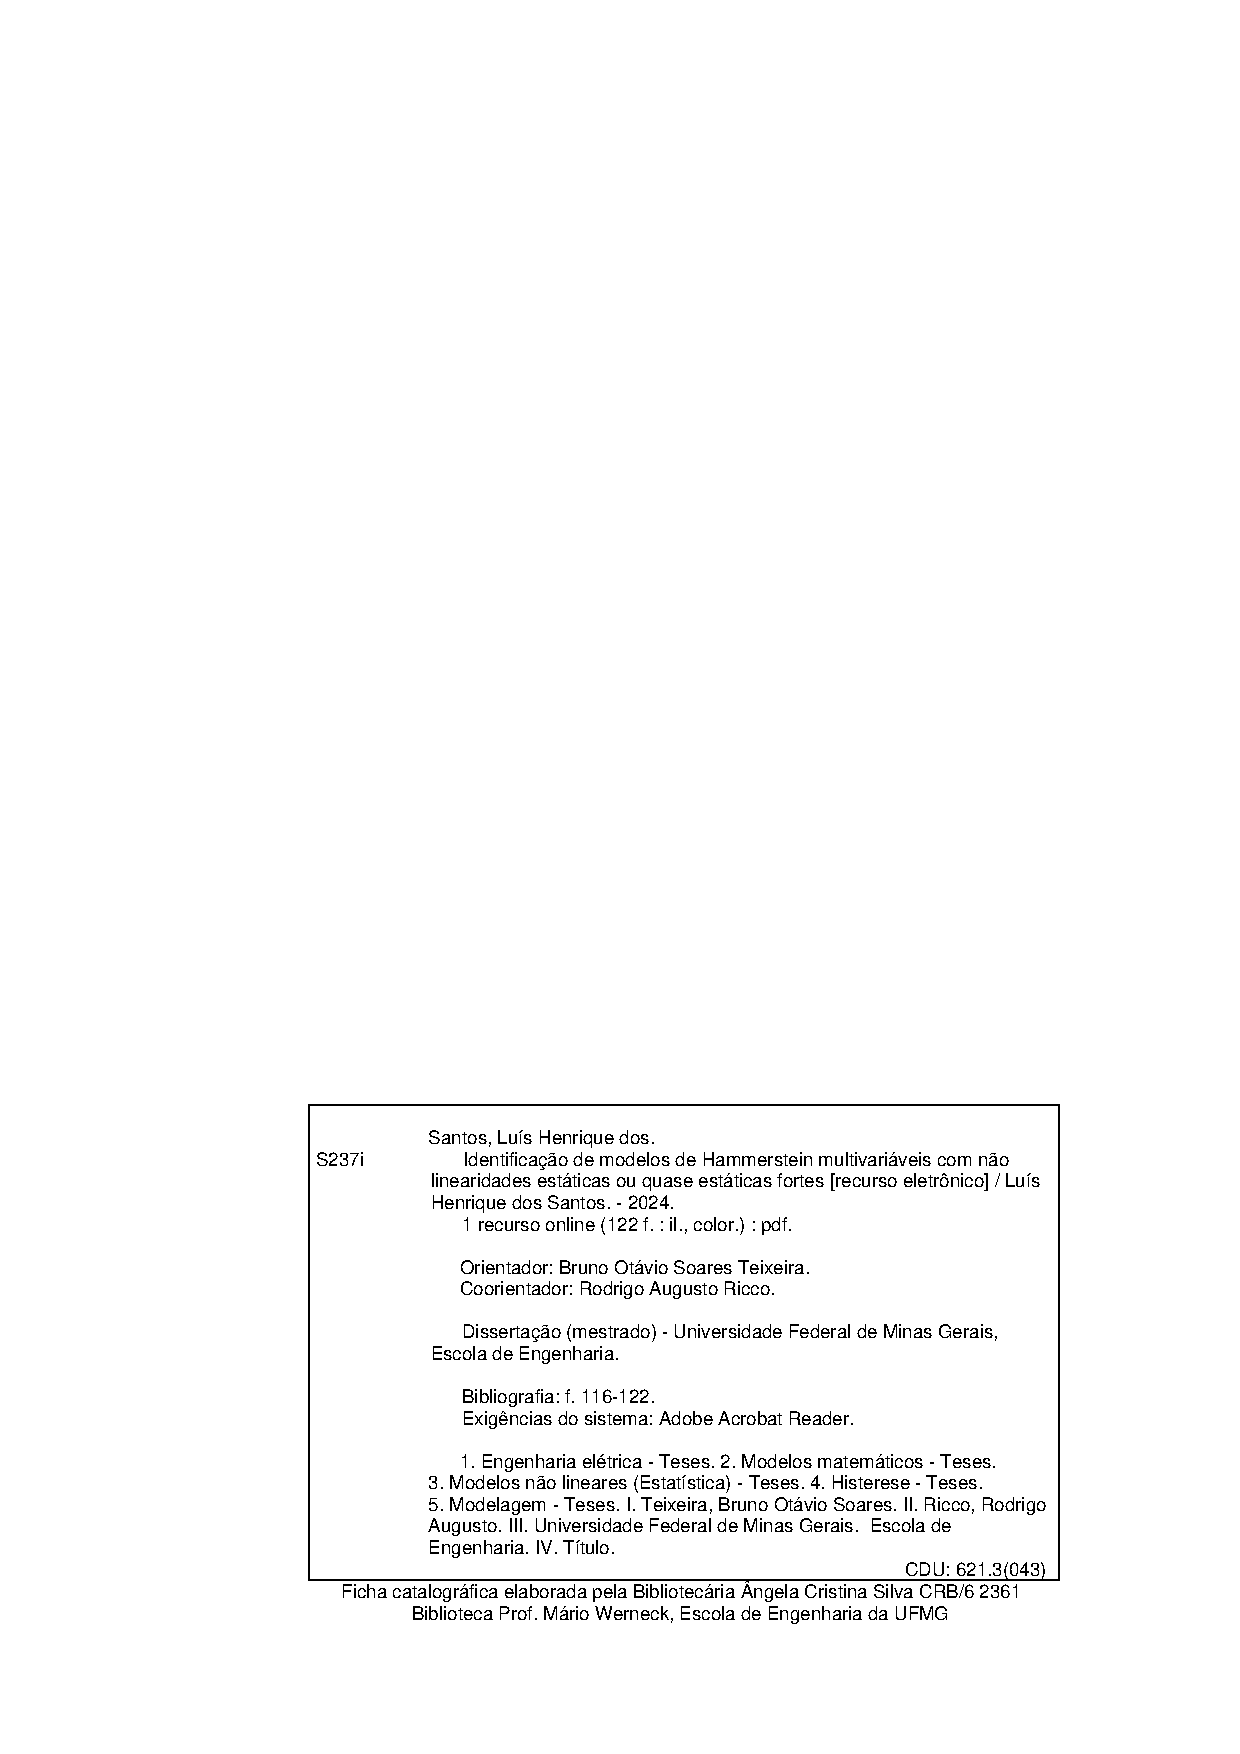
\includepdf[pages=-]{CATALOGRAFICA.pdf}

\includepdf[pages=-]{APROVACAO.pdf}

\pagestyle{empty} % retira algumas numerações de pagina
%--------------------------------------------------------------------
%Agradecimentos
\chapter*{Agradecimentos}
\thispagestyle{empty}
Em primeiro lugar, expresso minha gratidão à UFMG por ter me proporcionado toda uma estrutura de excelência, para a realização dos meus estudos. É através de instituições públicas de ensino superior como ela que podemos evoluir como sociedade. Estendo meus agradecimentos ao PPGEE-UFMG e aos seus funcionários, professores e alunos que contribuíram para o desenvolvimento deste trabalho. À Coordenação de Aperfeiçoamento de Pessoal de Nível Superior, CAPES, pelo suporte financeiro.


\clearpage
\thispagestyle{empty}
\cleardoublepage
%--------------------------------------------------------------------


%%--------------------------------------------------------------------
%%Epígrafe
%\chapter*{Epígrafe}


%\begin{flushright}
%\begin{minipage}{0.7\linewidth}
%\emph{``Fui átomo, vibrando entre as forças do Espaço,\\Devorando amplidões, em longa e ansiosa espera...\\Partícula, pousei... Encarcerado, eu era\\Infusório do mar em montões de sargaço.\\\\Por séculos fui planta em movimento escasso,\\Sofri no inverno rude e amei na primavera;\\Depois, fui animal, e no instinto da fera\\Achei a inteligência e avancei passo a passo...\\\\Guardei por muito tempo a expressão dos gorilas,\\Pondo mais fé nas mãos e mais luz nas pupilas,\\A lutar e chorar para, então, compreendê-las!...\\\\Agora, homem que sou, pelo Foro Divino,\\Vivo de corpo em corpo a forjar o destino\\Que me leve a transpor o clarão das estrelas!...''\\}
%\end{minipage}
%\end{flushright}
%%\vspace{3cm}
%\begin{flushright}
%{Soneto intitulado {\it Jornada}, de autoria de Adelino da Fontoura Chaves. Extraído do livro {\it Antologia dos Imortais}, psicografado por Francisco Cândido Xavier.}
%\end{flushright}

%"EVOLUÇÃO3
%
%                                                                                                              Rubens C. %Romanelli

%                De muito longe venho, em surtos milenários;

 %               Vivi na luz dos sóis, vaguei por mil esferas

  %              E, preso ao turbilhão dos motos planetários,

   %             Fui lodo e fui cristal, no alvor de priscas eras.

 

    %                            Mil formas animei, nos reinos multifários:

     %                           Fui planta no verdor de frescas primaveras

      %                          E, após sombrio estágio entre os protozoários,

       %                         Galguei novos degraus: fui fera dentre as feras.

 

        %        Depois que em mim brilhou o facho da razão,

         %       Fui o íncola feroz das tribos primitivas

          %      E como tal vivi, por vidas sucessivas.

 

           %                     E sempre na espiral da eterna evolução,
%
 %                               Um dia eu transporei os círculos do mal

  %                              E brilharei na luz da Essência Universal."

 % O Primado do Espírito
%\clearpage
%\thispagestyle{empty}
%\cleardoublepage
%%--------------------------------------------------------------------


%--------------------------------------------------------------------
%Resumo
%\begin{spacing}{1}
\chapter*{Resumo}
\thispagestyle{empty}
%\addcontentsline{toc}{chapter}{Resumo} \vspace{-0.5cm}

\noindent Os modelos descrevem características essenciais de sistemas, possibilitando análises e previsão de comportamentos que seriam dispendiosos, arriscados ou até mesmo impraticáveis. 
\par 
\noindent Palavras-chave: modelos de Hammerstein multivariáveis; não linearidades fortes; histerese; sistemas \textit{neuro-fuzzy}; modelo de Prandtl-Ishlinskii.


\clearpage
\thispagestyle{empty}
\cleardoublepage
%--------------------------------------------------------------------


%--------------------------------------------------------------------
%Abstract
\chapter*{Abstract}
\thispagestyle{empty}
%\addcontentsline{toc}{chapter}{Abstract}

\noindent Models describe essential characteristics of systems, enabling analysis and prediction of behaviors that would be expensive, risky or even impractical. 
\par
\noindent Keywords: multivariable Hammerstein models; strong nonlinearities; hysteresis; neuro-fuzzy systems; Prandtl-Ishlinskii model.
\clearpage
\thispagestyle{empty}
\cleardoublepage
%\end{spacing}
%--------------------------------------------------------------------


\begingroup % Essa parte também ajuda a tirar a numeração de list of figures
\makeatletter
\let\ps@plain\ps@empty
\makeatother

\pagestyle{empty}
\listoffigures
\cleardoublepage
\endgroup



%Abreviaturas
%--------------------------------------------------------------------
\chapter*{Lista de Abreviações}
\thispagestyle{empty}
%\addcontentsline{toc}{chapter}{Lista de Abreviações}


\begin{acronym}[MOESP-PO] %lembrar que o argumento opcional é o maior acrônimo utilizado %lembrar de manter a lista em ordem alfabética
	\acro{ARX}{modelo autorregressivo com entradas exógenas (\textit{AutoRegressive model with eXogenous inputs})}
	\acro{CVA}{análise de variáveis canônicas (\textit{Canonical Variate Analysis})}
	\acro{EIA-PSO}{otimização por enxame de partículas com estratégia adaptativa, informada e eficaz (\textit{Effective Informed Adaptive} - \textit{Particle Swarm Optimization})}
	\acro{EJL}{estrutura do modelo de Hammerstein proposta por Eskinat, Johnson e Luyben}
	\acro{GPI}{modelo de Prandtl-Ishlinskii generalizado (\textit{Generalized} Prandtl-Ishlinskii)}
	\acro{GRDPI}{modelo de Prandtl-Ishlinskii generalizado e dependente da taxa (\textit{Generalized Rate-Dependent} Prandtl-Ishlinskii)}
	\acro{KU}{estrutura do modelo de Hammerstein proposta por Kortmann e Unbehauen}
	\acro{LIT}{sistema Linear e Invariante no Tempo}
	\acrodefplural{LIT}{sistemaas Lineares e Invariantes do Tempo}
	\acro{LMI}{desigualde matricial linear (\textit{Linear Matrix Inequalitie})}
	\acrodefplural{LMI}{desigualdes matriciais lineares (\textit{Linear Matrix Inequalities})}
	\acro{MATLAB}{\textit{MATrix LABoratory}}
	\acro{MBI}{Modelo de Blocos Interconectados}
	\acrodefplural{MBI}{Modelos de Blocos Interconectados}
	\acro{MIMO}{múltiplas entradas e múltiplas saídas (\textit{Multiple Input Multiple Output})}
	\acro{MISO}{múltiplas entradas e uma saída (\textit{Multiple Input Single Output})}
	\acro{MOESP}{modelo multivariável de erro na saída em espaço de estados (\textit{Multivariable Output-Error State sPace})}
	\acro{MOESP-PO}{modelo multivariável de erro na saída em espaço de estados com entradas passadas atuando como variáveis instrumentais (\textit{Multivariable Output-Error State sPace - Past Output})}
	\acro{MPSO}{otimização por enxame de partículas modificado (\textit{Modified Particle Swarm Optimization})}
	\acro{MQ}{Mínimos Quadrados}
	\acro{N4SID}{Algoritmos numéricos para identificação de sistema em espaço de estados empregando técnicas de subespaço (\textit{Numerical algorithms for Subspace State-Space System IDentification})}
	\acro{NARMAX}{modelo média móvel autoregressivo não linear com entrada exógena (\textit{Nonlinear AutoRegressive Moving Average with eXogenous input})}
	\acro{NARX}{modelo autoregressivo não linear com entrada exógena (\textit{Nonlinear AutoRegressive with eXogenous input})}
	\acro{NF}{\textit{Neuro-Fuzzy}}
	\acro{PBSID}{método de identificação por subespaço baseado em preditor (\textit{Predictor-Based Subspace IDentification method})}
	\acro{PEM}{método de predição de erro (\textit{Prediction Error Method})}
	\acro{P-I}{Prandtl-Ishlinskii}
	\acro{PRBS}{sinal binário pseudoaleatório (\textit{Pseudo Random Binary Signal})}
	\acro{PSO}{otimização por enxame de partículas (\textit{Particle Swarm Optimization})}
	\acro{RDPI}{modelo de Prandtl-Ishlinskii dependente da taxa (\textit{Rate-Dependent} Prandtl-Ishlinskii)}
	\acro{RMSE}{raiz quadrada do erro médio quadrático (\textit{Root Mean Square Error})}
	\acro{SBAI}{Simpósio Brasileiro de Automação Inteligente}
	\acro{SIMO}{uma entrada e múltiplas saídas (\textit{Single Input Multiple Output})}
	\acro{SISO}{uma entrada e uma saída (\textit{Single Input Single Output})}
	\acro{SNR}{relação sinal ruído (\textit{Signal Noise Ratio})}
	\acro{SVD}{decomposição em valores singulares (\textit{Singular Value Decomposition})}
\end{acronym}
\clearpage
\thispagestyle{empty}
\cleardoublepage
%\end{spacing}
%--------------------------------------------------------------------



%--------------------------------------------------------------------
%Símbolos
%--------------------------------------------------------------------
\chapter*{Lista de Símbolos}
\thispagestyle{empty}
%\addcontentsline{toc}{chapter}{Lista de Símbolos}


\begin{itemize}[leftmargin=30pt,labelsep=1em,align=left]
	\setlength\itemsep{0em}
	\item[$\in$] Pertence;
	\item[$\mathbb{R}$] Conjunto dos número reais;
	\item[$p$] Quantidade de entradas de processos ou modelos de blocos interconectados;
	\item[$k$] Variável de tempo discreto;
	\item[$u(k)$] Entrada de sistemas não autônomos no instante $k$, $u(k) \in \mathds{R}^{p}$;
	\item[$\varrho$] Quantidade de sinais intermediários de processos ou modelos de blocos interconectados;
	\item[${v}(k)$] Sinal intermediário dos modelos de blocos interconectados no instante $k$, $v(k)~\in~\mathds{R}^{\varrho}$;
	\item[$m$] Quantidade de saídas de processos ou modelos de blocos interconectados;
	\item[$y(k)$] Sinal de saída dos modelos no instante $k$, $y(k)  \in \mathds{R}^{m}$;
	\item[$\mathcal{N}$] Não linearidades do processo ou do modelo de blocos interconectados;
	\item[$\mathcal{L}$] Parcela linear do processo ou do modelo de blocos interconectados;
	\item[$x(k)$] Vetor de estados no instante $k$, $x(k)  \in \mathds{R}^{n}$;
	\item[$A$] Matriz da dinâmica do sistema $ \in \mathds{R}^{n \times n}$;
	\item[$B$] Matriz de entradas $ \in \mathds{R}^{n \times \varrho}$;
	\item[$C$] Matriz de saída $ \in \mathds{R}^{m \times n}$;
	\item[$D$] Matriz de transmissão direta $ \in \mathds{R}^{m \times \varrho}$;
	\item[$w(k)$] Vetor de ruído de medição $ \in \mathds{R}^{n}$;
	\item[$\mathcal{T}$] Transformação de similaridade;
	\item[$\hat{(\bullet)}$] Estimativa de $(\bullet)$;
	\item[$i$] Índice que assume valores de 1 a $p$;
	\item[$\textrm{\footnotesize \cursive \textit{f}}\,(\cdot)$] Função crisp;
	\item[$\vartheta$] Parâmetro consequente do modelo Takagi-Sugeno de ordem zero;
	\item[$c$] Centro de uma função de pertinência gaussiana;
	\item[$\sigma$] Dispersão de uma função de pertinência gaussiana;
	\item[$t$] Variável de tempo contínuo;
	\item[$b_\bullet$] Parâmetros do modelo de Bouc-Wen;
	\item[$\dot{\bullet}$] Derivada de $\bullet$ no tempo contínuo;
	\item[$d_\bullet$] Parâmetros do modelo de Duhem;
	\item[$p_\bullet$] Disparo do operador elementar de Preisach ;
	\item[$N_P$] Quantidade de operadores no modelo de Prandtl-Ishlinskii;
	\item[$\mathcal{S}$] Operador elementar \textit{stop};
	\item[$r$] Disparo de um operador elementar de Prandtl-Ishlinskii;
	\item[$j$] Índice que assume valores de 1 a $N_P$;
	\item[$\theta$] Parâmetro dos operadores do modelo de Prandtl-Ishlinskii;
	\item[$\mathcal{P}$] Operador elementar \textit{play};
	\item[$\mathcal{B}$] Função de borda do operador \textit{play};
	\item[$\mathcal{G}$] Operador \textit{play} generalizado;
	\item[$\mathfrak{b}$] Parâmetros da função de borda;
	\item[$\breve{\theta}$] Parâmetro dos disparos dinâmicos do modelo de Prandtl-Ishlinskii;
	\item[$T_s$] Período de amostragem;
	\item[$p_n$] Ordem de persistência de excitação;
	\item[$P_N$] Número de colunas da matriz $\mathcal{V}$;
	\item[$h$] Quantidade de blocos linha de uma matriz em blocos de Hankel;
	\item[$\Gamma$] Matriz de observabilidade estendida;
	\item[$T$] Transposto;
	\item[$N_L$] Quantidade de dados para identificar dinâmica linear;
	\item[$\mathscr{V}$] Matriz em bloco de Hankel equacionada com $v(k)$;
	\item[$\Upsilon$] Matriz em bloco de Hankel equacionada com $y(k)$;
	\item[$R$] Matriz à esquerda da fatoração RQ;
	\item[$Q$] Matriz à direita da fatoração RQ;
	\item[$U_o$] Matriz à esquerda da decomposição em valores singulares;
	\item[$S_o$] Matriz com valores singulares da decomposição em valores singulares;
	\item[$V_o$] Matriz à direita da decomposição em valores singulares;
	\item[$l$] Índice que assume valores de 1 a $m$;
	\item[$N_N$] Quantidade de dados para identificar a não linearidade;
	\item[$G_\mathcal{N}$] Ganho em regime de uma parcela estática não linear do modelo de Hammerstein;
	\item[$G_\mathcal{L}$] Ganho em regime de uma parcela dinâmica linear do modelo de Hammerstein;
	\item[$G_\mathcal{NL}$] Ganho em regime de um modelo de Hammerstein;
	\item[$\beta$] Ganho de uma função estática não linear no ponto $u_\beta$;
	\item[$I_\bullet$] Matriz identidade de ordem $\bullet$; 
	\item[$N_N^{(i)}$] Quantidade de dados do ensaio estático realizado na entrada $i$;
	\item[$\bar{N}_{i,j}$] Quantidade de dados formando o $j$-ésimo \textit{cluster} da entrada $i$;
	\item[$N_i$] Quantidade total de \textit{clusters} para a entrada $i$;
	\item[$\mathscr{J}$] Indica a posição do \textit{cluster} mais próximo do dado $u_i(k)$;
	\item[$S_{i,0}$] Abrangência do \textit{cluster} $i$;
	\item[$\lambda$] Fator de deslocamento do centro do \textit{cluster};
	\item[$\rho$] Controle da dispersão da gaussiana;
	\item[$E$] Função custo da metodologia \textit{neuro-fuzzy};
	\item[$\Phi$] Ponderação utilizada na defuzificação;
	\item[$\mu$] Função gaussiana;
	\item[$n_d$] Ordem a partir da qual a derivada parcial de $E$ é nula;
	\item[$n_p$] Número de estágios do registrador para gerar um sinal binário pseudoaleatório;
	\item[$\mathbb{N}$] Conjunto dos números naturais;
	\item[$\mathscr{U}$] Distribuição uniforme;
	\item[$\mu_u$] Média da distribuição uniforme;
	\item[$\sigma_u$] Desvio padrão da distribuição uniforme;
	\item[$\mathscr{N}$] Distribuição normal;
	\item[$\mu_n$] Média da distribuição normal;
	\item[$\sigma_n$] Desvio padrão da distribuição normal;
	\item[$\iota$] Índice que assume valores de 1 a $\varrho$;
	\item[$\mathcal{GR}$] Operador \textit{play} generalizad dependente da taxa;
	\item[$\Theta$] Parâmetros do operador $\mathcal{GR}$;
	\item[$N_V$] Quantidade total de parâmetros de $\Theta$;
	\item[$F$] Função de aptidão das partículas de uma nuvem;
	\item[$V$] Matriz com a velocidade das partículas de uma nuvem;
	\item[$\tilde{\theta}$] Parâmetros que controlam a função de borda do operador generalizado dependente da taxa de Prandtl-Ishlinkii;
	\item[$\epsilon$] Parâmetro interno do modelo GRDPI;
	\item[$\Delta u$] Variação entre amostras do sinal de entrada;
	\item[$N_G$] Quantidade de dados usados para ajustar o ganho total do modelo de Hammerstein MIMO GRDPI;
	\item[$\xi$] Quantidade de partículas selecionadas para compor o grupo de melhores partículas no PSO;
	\item[$K_{\mu}$] Quantidade de iteração que iterações consecutivas sem alteração da função custo $F(\Theta)$ a partir da qual podem ocorrer mutações;
	\item[$P$] Quantidade de partículas do PSO;
	\item[$\ell$] Índice que assume valores de 1 a $P$;
	\item[$\kappa$] Índice da atual iteração do PSO;
	\item[$K_{\max}$] Quantidade de iterações que o PSO é executado;
	\item[$\alpha$] Probabilidade de ocorrer mutação no PSO;
	\item[$\varpi$] Taxa de aprendizado cognitivo e social do PSO;
	\item[$U$] Matriz com amostras da distribuição uniforme;
	\item[$\odot$] Multiplicação elemento a elemento;
	\item[$M^{(p)}$] Média ponderada das melhores posições pessoais;
	\item[$M^{(g)}$] Média ponderada das melhores posições globais;
	\item[$\varsigma$] Média ponderada das melhores funções de aptidão;
	\item[$q$] Índice que assume valores de 1 a $\xi$ independente de $g$;
	\item[$g$] Índice que assume valores de 1 a $\xi$ independente de $q$;
	\item[$s$] Índice que assume valores de 2 a $P$;
	\item[$\chi$] Fator de constrição do PSO;
	\item[$\nu$] Amostra de uma distribuição uniforme;
	\item[$\gamma$] Uma dimensão aleatória de velocidade $V$;
	\item[$\eta$] Índice aleatório que indica uma das $P$ partículas da nuvem;
	\item[$\zeta$] Fator aleatório que altera a velocidade de uma partícula;
	\item[$\overline{b}$] Nível superior de um sinal PRBS;
	\item[$\underline{b}$] Nível inferior de um sinal PRBS;
	\item[$\overline{\theta}$] Ganhos da parte superior do sinal intermediário;
	\item[$\underline{\theta}$] Ganhos da parte inferior do sinal intermediário;
	\item[$\underline{\Theta}$] Matriz de parâmetros com ganhos do sinal intermediário a serem otimizados;
	\item[$\underline{v}$] sinal intermediário compensado com os ganhos $\underline{\Theta}$;
	\item[$\underline{y}$] sinal intermediário compensado com os ganhos $\underline{\Theta}$;
	\item[$\underline{\mathcal{L}}$] Estimativa inicial do bloco dinâmico linear.
\end{itemize}


\clearpage
\thispagestyle{empty}
\cleardoublepage
%--------------------------------------------------------------------

%%--------------------------------------------------------------------
%Sumário
\begingroup % Essa parte também ajuda a tirar a numeração de list of figures
\makeatletter
\let\ps@plain\ps@empty
\makeatother

\pagestyle{empty}
\tableofcontents
\cleardoublepage
\endgroup

%\pagestyle{myheadings}
%\begin{spacing}{1.5}

%\end{spacing}
%\clearpage
%\thispagestyle{empty}
%\cleardoublepage

\pagestyle{plain} % volta com a numeração de paginas

%Esse já estava comentado antes que eu comentasse os de baixo %Lista de Tabelas 
%Esse já estava comentado antes que eu comentasse os de baixo %\begin{spacing}{1.5}
%\listoftables
%\addcontentsline{toc}{chapter}{Lista de Tabelas}
%\clearpage
%\thispagestyle{empty}
%\cleardoublepage



%Começando os capítulos
%--------------------------------------------------------------------
\clearpage
\pagestyle{myheadings}
%\pagenumbering{arabic}
%--------------------------------------------------------------------

%--------------------------------------------------------------------
%Definição de cabeçalhos
\pagestyle{fancy}
\renewcommand{\chaptermark}[1]{\markboth{\thechapter\ #1}{}}
\renewcommand{\sectionmark}[1]{\markright{\thesection\ #1}{}}
\fancyhf{}
\fancyhead[LE,RO]{\thepage}
\fancyhead[LO]{\rightmark}
\fancyhead[RE]{\leftmark}
\renewcommand{\headrulewidth}{0.5pt}
\renewcommand{\footrulewidth}{0.0pt}
\addtolength{\headheight}{2.5pt}                % 2.5pt
\fancypagestyle{plain}{
     \fancyhead{}
     \renewcommand{\headrulewidth}{0pt}
     }
     
     

%--------------------------------------------------------------------
%Capítulo 1 - Introdução
\chapter{Introdução}
\label{cap:intro} \vspace{-1cm} \vspace{1cm}


%\section{Considerações iniciais} \markright{\thesection ~~~ Considerações iniciais}
%\label{sec:intro_inicial}
\section{Motivação e Justificativa} \markright{\thesection ~~~ Motivação e Justificativa}
\label{sec:intro_motiva}
%
\par
A identificação de sistemas dedica-se a obter um modelo matemático para um sistema dinâmico por meio de dados experimentais. Em geral, esses dados são observados com ruído em um sistema físico completamente desconhecido ou com determinadas características desconhecidas. O objetivo do modelo é aproximar propriedades específicas de um sistema e não necessariamente criar um modelo genérico que o represente completamente em qualquer situação. Como escrito por George Box, ``essencialmente, todos os modelos estão errados, mas alguns são úteis''~(\citealp{box1987}, p. 424, tradução própria\footnote{No original: ``Essentially, all models are wrong, but some are useful.''}), ou seja, o propósito de construir o modelo é que ele sirva para determinada tarefa e não que ele seja um modelo de tudo. Desse modo, é pertinente atestar se um modelo linear descreve o sistema da maneira desejada antes de partir para a abordagem não linear.
\par 
Uma das principais etapas do procedimento de identificação de um sistema é a seleção da estrutura que o modelo apresentará, na qual é essencial considerar a linearidade do elemento sob investigação~\citep{aguirre2015,nelles2020}. Na prática, nenhum processo ou componente é linear, no entanto, quando os sinais de interesse que o descrevem permanecem em torno de um ponto de operação, o sistema pode ser analisado e, eventualmente, modelado sob a suposição de linearidade. Ainda assim, por mais que o modelo linear seja uma aproximação local, ele pode ser eficaz em regiões mais amplas à medida que as não linearidades presentes e a precisão exigida são reduzidas. Desse modo, os modelos lineares constituem uma abordagem amplamente utilizada~\citep{sastry2013}. Tendo em vista a complexidade dos sistemas, que, por vezes, são multivariáveis, uma representação adequada é o modelo linear em espaço de estados, conveniente para estimação, filtragem, predição e controle. Eles podem ser obtidos empregando os métodos de identificação por subespaços que podem estimar modelos no espaço de estados para sistemas multivariáveis por meio de dados de entrada e saída~\citep{katayama2005,van2012}. 
\par 
Observe as ilustrações da Figura~\ref{fig:cap1naolinearidade} que retratam duas curvas não lineares aproximadas por retas, em que cada reta é um modelo diferente. Dentre as duas curvas, aquela exibida em~a) possui menor variação, por isso pode ser representada por três retas. Por outro lado, a curva apresentada em~b) precisou de treze retas no mesmo intervalo de entrada para ter uma aproximação qualitativamente próxima a~b). À vista disso, a quantidade de modelos a serem gerenciados no caso apresentado na imagem b) é maior e mais custosa de implementar. Nessas circunstâncias, nota-se que modelos lineares podem ser ineficientes quando se deseja operar o processo em faixas amplas. A informação transmitida é que, para determinados sistemas, a representação por modelos lineares pode não ser uma alternativa atraente. Portanto, descartada a possibilidade de utilizar um modelo linear, pode-se adotar representações não lineares para analisar, prever o comportamento ou controlar o sistema sob estudo. Como os problemas não lineares costumam ser específicos, é comum que os métodos tratem de maneira particular cada tipo de não linearidade, aumentando os obstáculos de modelagem. 
%
\begin{figure}[htb]
	\centering
	\label{fig:cap1naolinearidade}
	\begin{tabular}{cc}
		a) & b)\\
		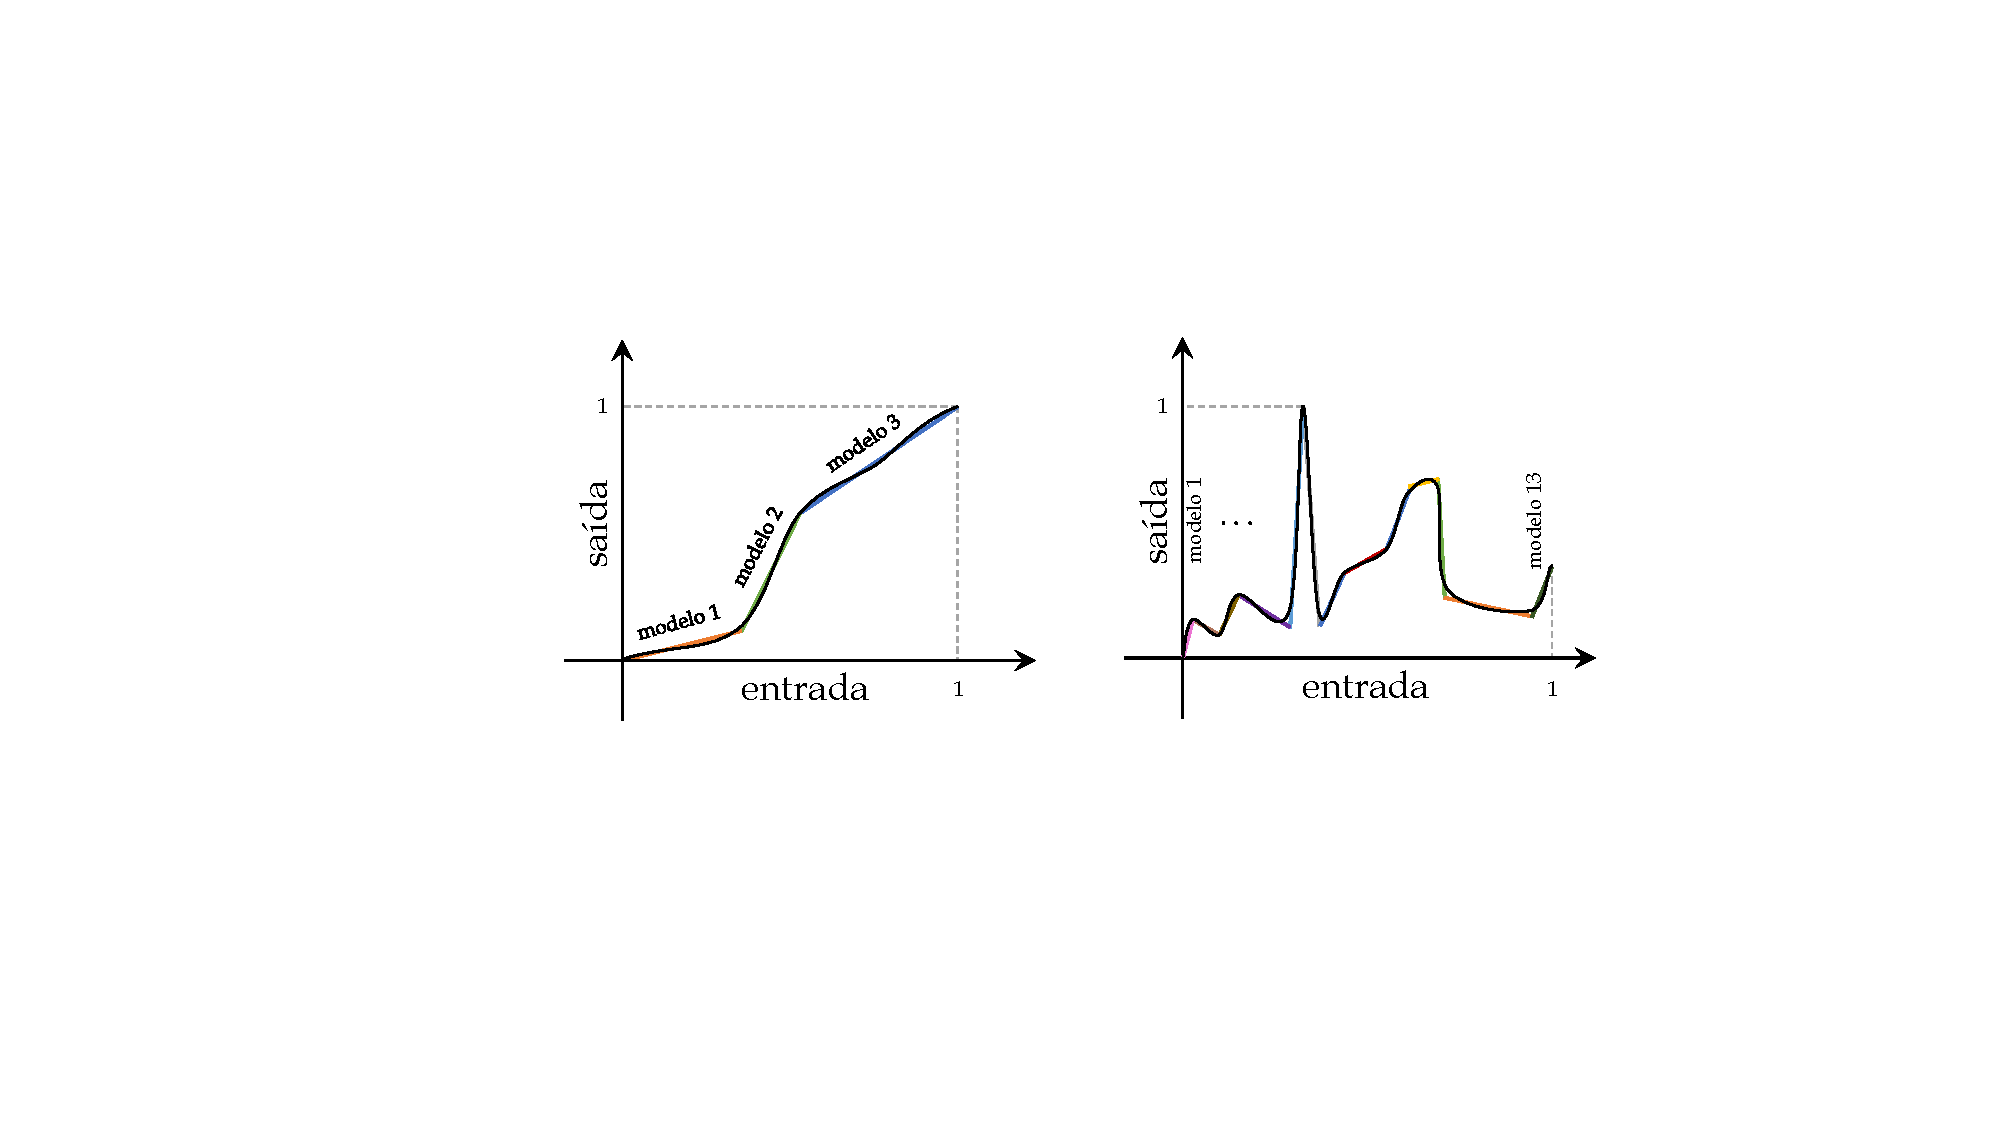
\includegraphics[scale=0.6,trim=85mm 70mm 150mm 55mm,clip=true]{figuras/cap1naolinearidade} &
		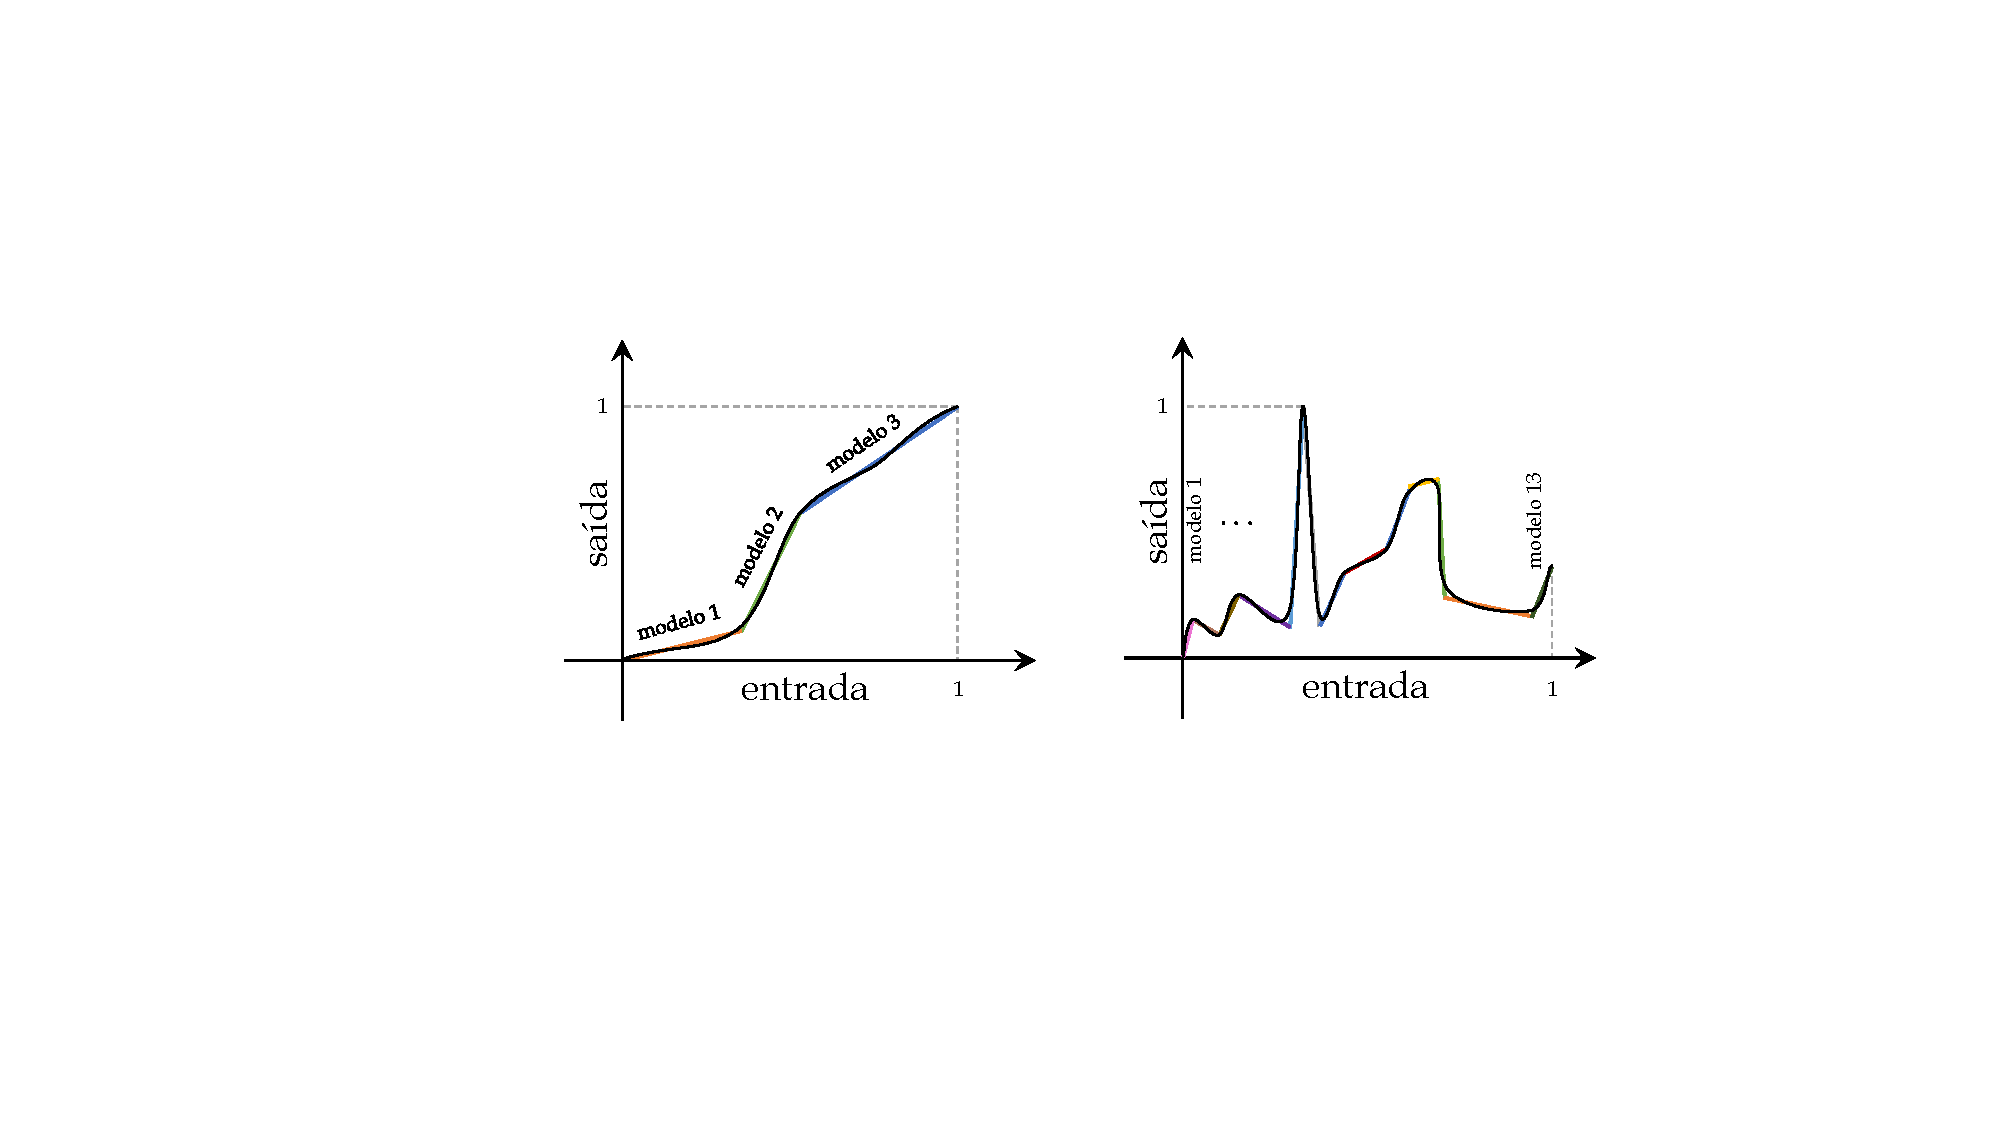
\includegraphics[scale=0.6,trim=176mm 70mm 50mm 55mm,clip=true]{figuras/cap1naolinearidade}
	\end{tabular}
	\caption[Curva estática não linear representada por retas, sendo cada reta a representação de um modelo diferente.]{Curva estática não linear representada por retas, sendo cada reta a representação de um modelo diferente. Em~a) é desenhada uma curva não linear que foi aproximada por três retas e em~b) está uma curva com diversas sinuosidades de modo que foram necessárias treze retas para representar a curva~b) de maneira qualitativamente próxima ao que foi feito com a curva em~a).}
\end{figure}
\par 
A busca por uma representação matemática para sistemas não lineares levou ao desenvolvimento de técnicas para a modelagem baseadas em séries funcionais, como as séries de Volterra. Porém, elas são complexas do ponto de vista computacional e geram dificuldade na inserção de informação \textit{a priori}~\citep{borjas2013}. Estruturas que surgiram posteriormente incluem, por exemplo: modelos \acs{NARMAX} (do inglês \textit{Nonlinear AutoRegressive Moving Average with eXogenous input})~\citep{billings2013}, modelos \textit{Neuro-Fuzzy} (\acs{NF})~\citep{nelles2020}, modelos de blocos interconectados~\citep{mzyk2014}, modelos não paramétricos~\citep{ljung2010}, entre outros. 
\par 
No decorrer deste trabalho o foco será dado aos modelos de blocos interconectados (\acsp{MBI}) que consistem na junção de subsistemas dinâmicos lineares invariantes no tempo (\acs{LIT}) e elementos estáticos não lineares. As estruturas clássicas de blocos interconectados consistem na conexão em série entre os  blocos linear e não linear. Elas recebem o nome de modelo de Hammerstein ou Wiener a depender da disposição desses blocos. Apesar da sua simplicidade, os modelos de Hammerstein e Wiener provaram poder descrever com precisão uma ampla variedade de sistemas não lineares, por exemplo, processos químicos~\citep{zou2015,roy2016,li2016}, biológicos~\citep{kian2013,fracz2016}, biomédicos~\citep{kian2013,najafabadi2016} e também em identificação para controle~\citep{biagiola2016,zhang2017,rayouf2018,li2022}.
\par 
No fim da década de 1980, surgiram os métodos de identificação por subespaços. Esses métodos foram formulados sob diversas perspectivas, tais como, \acs{CVA} (do inglês \textit{Canonical Variate Analysis})~\citep{larimore1990}, \acs{N4SID} (do inglês \textit{Numerical algorithms for Subspace State Space System IDentification})~\citep{van1994} e \acs{MOESP} (do inglês \textit{Multivariable Output Error State sPace})~\citep{verhaegen1992a,verhaegen1992b}. Essas técnicas puderam ser aplicadas para identificação da dinâmica linear dos modelos de blocos interconectados em espaço de estados. Trabalhos como os de~\citep{gomez2005},~\citep{depaula2015} e~\citep{santos2021}, empregam o \acs{MOESP} para identificar as dinâmicas lineares associadas aos modelos de Hammerstein e Wiener em processos com não linearidades suaves.
\par
Uma distinção que pode ser feita entre as curvas não lineares diz respeito à suavidade. Uma função suave possui derivada contínua em qualquer ponto do seu domínio, como é o caso daquelas apresentadas em preto contínuo na Figura~\ref{fig:cap1naolinearidade}a). Por outro lado, quando há ao menos um ponto em que a derivada não está definida, tem-se uma não linearidade definida como não linearidade forte. 
%
\begin{definicao}
	Uma função não linear forte é aquela em que a derivada não está definida em pelo menos um ponto no seu domínio. 
\end{definicao}
%
Exemplos de não linearidades fortes que se manifestam frequentemente em sistemas práticos incluem histerese, saturação, zona morta e folga~\citep{grimble2020}. Três delas são apresentadas na Figura~\ref{fig:cap1_hist_sat_zmorta}. 
%
\begin{figure}[htb]
	\centering
	\begin{tabular}{ccc}
		a) & b) & c)\\
		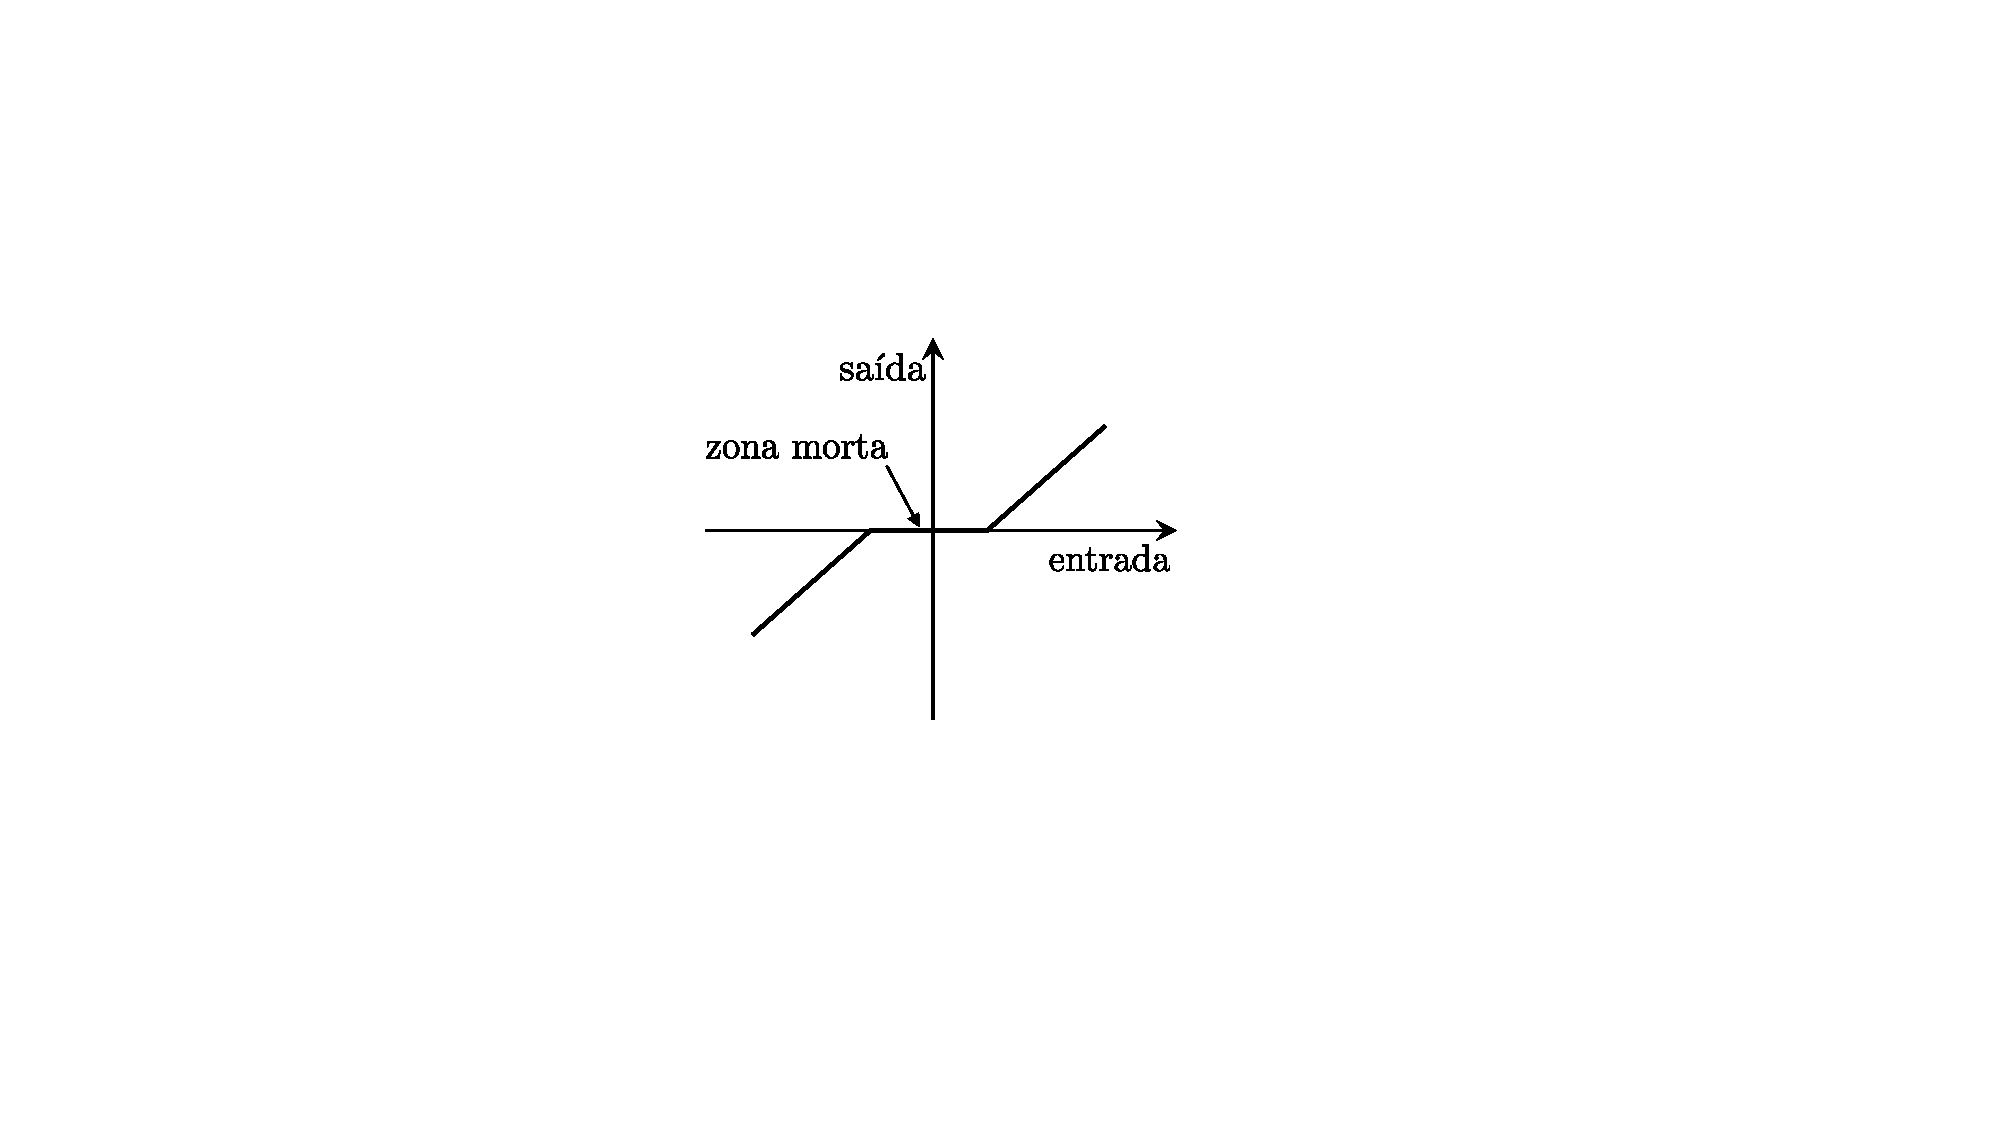
\includegraphics[scale=0.56,trim=115mm 70mm 135mm 55mm,clip=true]{figuras/cap1_zona_morta} &
		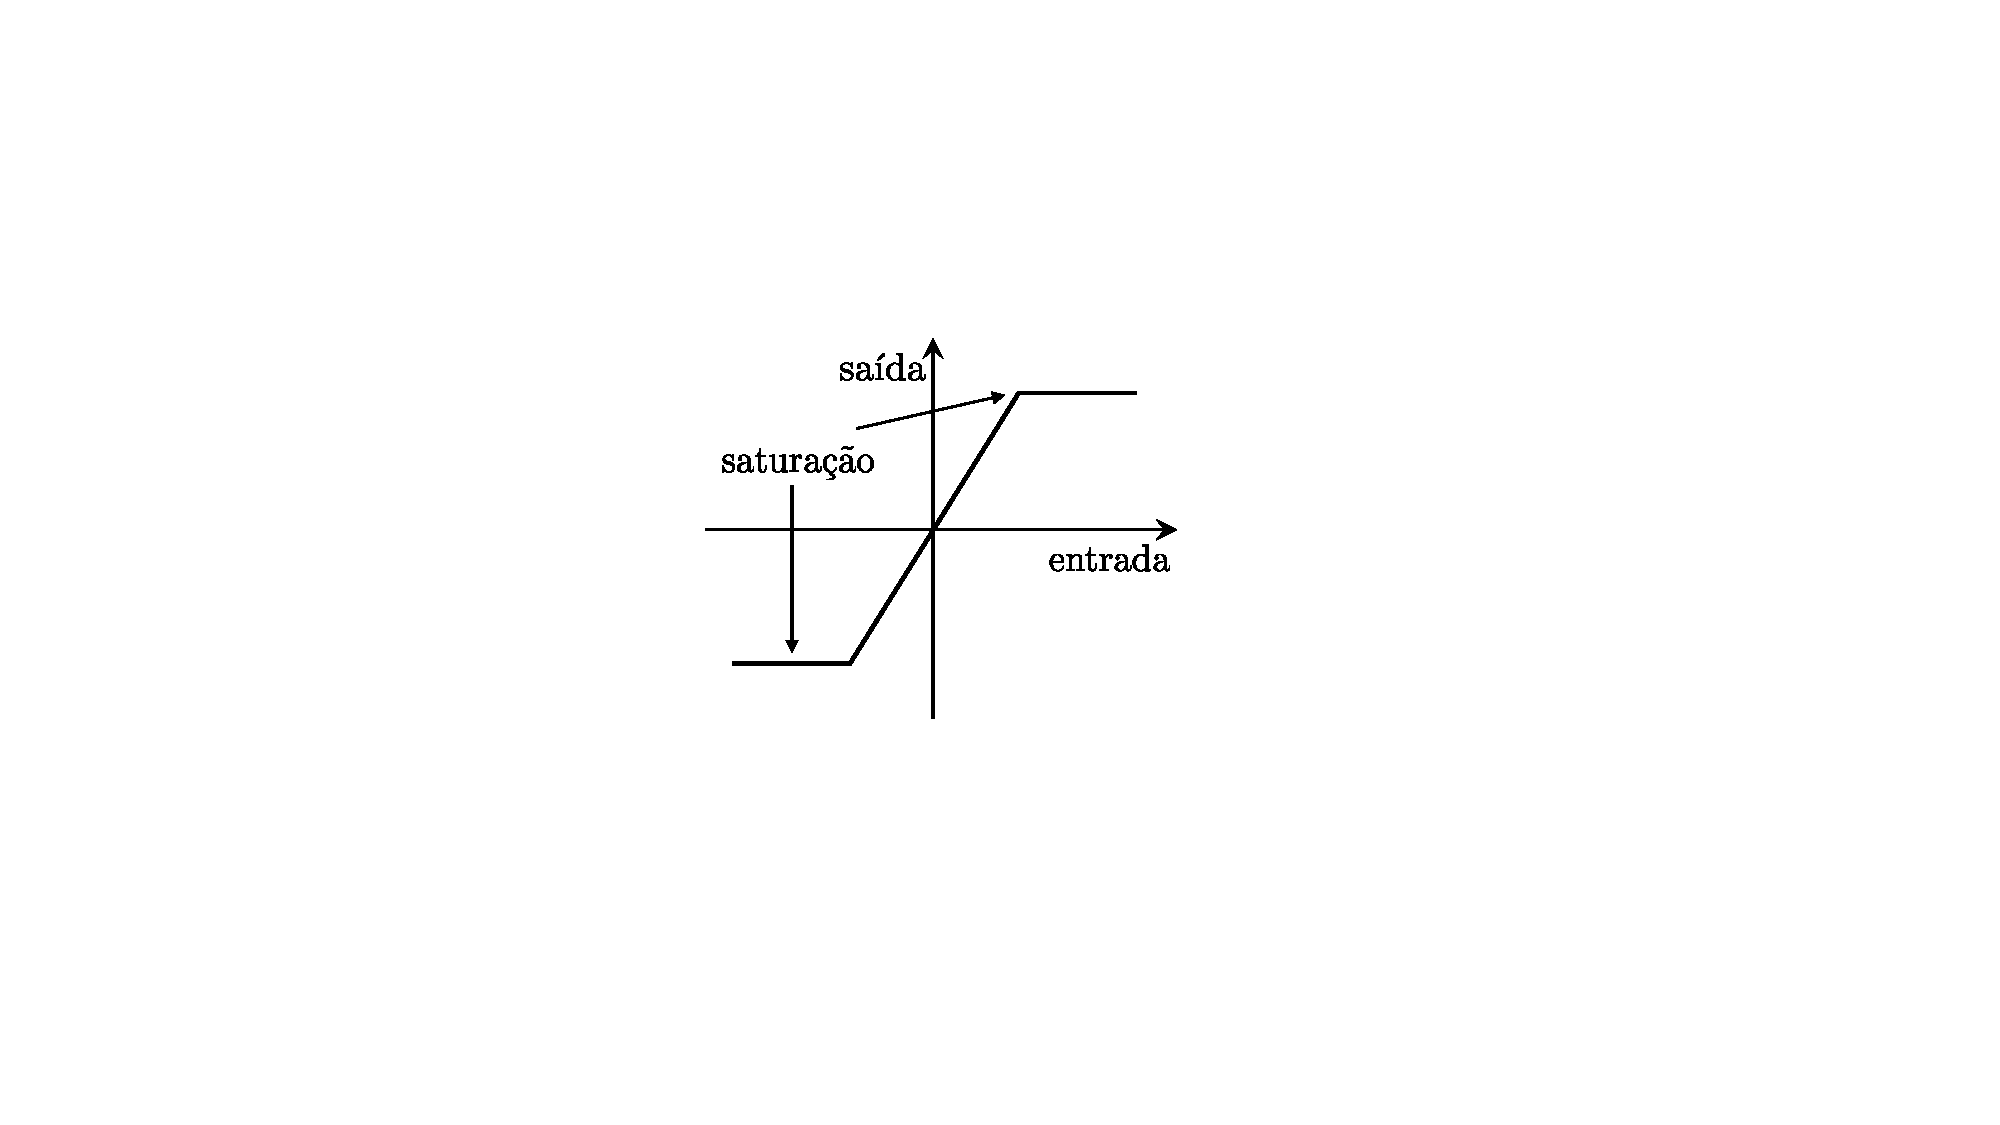
\includegraphics[scale=0.56,trim=115mm 70mm 135mm 55mm,clip=true]{figuras/cap1_saturacao} &
		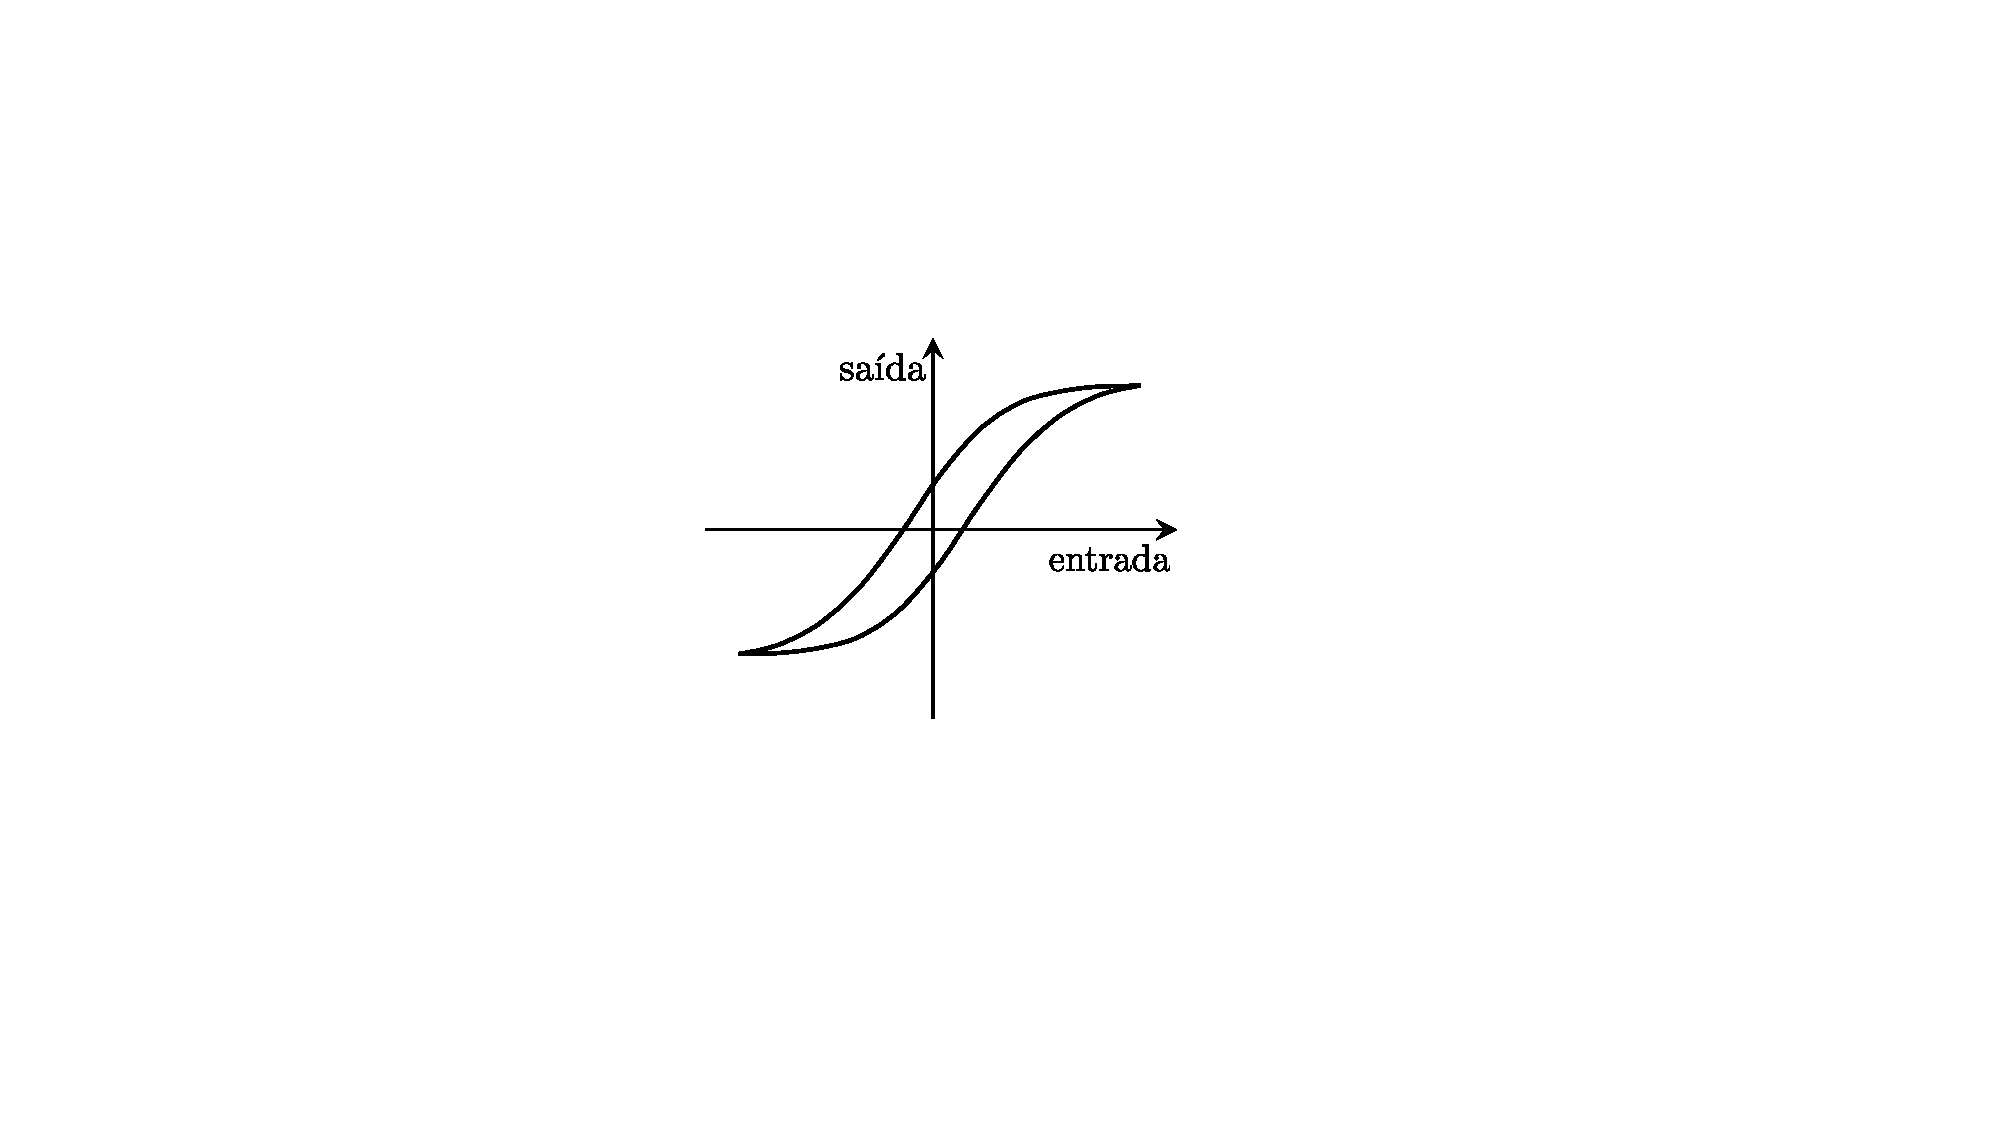
\includegraphics[scale=0.56,trim=115mm 70mm 135mm 55mm,clip=true]{figuras/cap1_histerese}
	\end{tabular}
	\caption[Exemplos de não linearidades fortes.]{Exemplos de não linearidades fortes. Em~a) apresenta-se a zona morta, em ~b) a saturação e em~c) a histerese.}
	\label{fig:cap1_hist_sat_zmorta}
\end{figure}
%
\par
Sistemas físicos, sejam eles mecânicos, elétricos, fluídicos, entre outros, podem apresentar não linearidades fortes. Por exemplo, as máquinas elétricas e transformadores possuem não linearidades na forma de saturação. Tais efeitos surgem quando núcleos ferromagnéticos estão presentes, uma vez que eles são descritos por curvas e equações de magnetização não lineares~\citep{fitzgerald2003}. Por sua vez, os sistemas mecânicos podem incluir não linearidades como zona morta, histerese e folga. A presença dessas não linearidades em sistemas mecânicos deve-se ao desgaste ou até mesmo aos limites físicos de percurso dos componentes. As não linearidades das válvulas são frequentes em plantas industriais, porém, um exemplo de não linearidade severa em sistemas fluídicos é a ação de relé comumente encontrada em processos de controle de nível~\citep{garcia2013}. 
\par
Devido à capacidade de modelar uma função estática não linear com precisão, alguns trabalhos utilizam redes neurais e sistemas \textit{fuzzy} para representar o elemento não linear dos modelos de Hammerstein. Em geral, as investigações dedicam-se à identificação de um mapeamento não linear global a partir de dados, porém, o resultado apresentado por~\cite{jia2005} foi obtido ao propor identificar separadamente a curva estática com uma rede \acs{NF} e a dinâmica linear utilizando o método clássico de mínimos quadrados. O sucesso da separação está relacionado ao emprego do sinal de teste proposto por~\cite{sung2002} que desacopla a identificação das partes lineares e não lineares. 
\par
A metodologia apresentada em~\citep{jia2005} foi desenvolvida para o caso monovariável. Posteriormente, o caso multivariável foi desenvolvido em~\citep{jia2016}, usando-se técnicas de inteligência computacional para identificar a curva não linear sob a forma de uma rede \acs{NF} e um algoritmo de análise de correlação para estimar os parâmetros da dinâmica linear sob a forma de um modelo  autorregressivo com entradas exógenas (\acs{ARX}, do inglês \textit{AutoRegressive with eXogenous input}). Entretanto, para sistemas multivariáveis, a representação em espaço de estados é a mais adequada. 
\par 
O comportamento não linear estudado em~\citep{jia2005} e~\citep{jia2016} é estático e forte dada a presença de descontinuidades nas curvas identificadas. Apesar dos avanços nas últimas décadas, a literatura relacionada ao uso de métodos de subespaços para obtenção de modelos representados no espaço de estados para sistemas não lineares multivariáveis é escassa, sobretudo quando se tratam de não linearidades fortes. Dessa maneira, propõe-se, nesta dissertação, uma nova abordagem para identificar modelos de Hammerstein de várias entradas e várias saídas (\acs{MIMO}, do inglês \textit{Multiple Input Multiple Output}) com não linearidades fortes, empregando técnicas de inteligência computacional aliadas ao algoritmo \acs{MOESP}~\citep{verhaegen1992a}. Busca-se identificar uma rede \acs{NF} que represente a curva estática não linear e um modelo em espaço de estados que exprima a dinâmica linear sem a necessidade de qualquer conhecimento prévio. Isso é possível, pois o \acs{MOESP} é capaz de retornar as matrizes e a ordem do sistema, sem exigir a escolha prévia da estrutura do modelo~\citep{verhaegen1992a}. Além disso, a rede \acs{NF} evita restrições à função não linear estática, encontradas usando a abordagem polinomial~\citep{jia2005}, e não apresenta problemas de inicialização, como outros algoritmos iterativos~\citep{Chen2011}.
\par 
Outro comportamento não linear forte de interesse é a histerese. Ela está presente em diversos sistemas mecânicos industriais, manifestada em sensores e atuadores como os piezoelétricos e válvulas de controle pneumático~\citep{abreu2020}. Essa não linearidade é um fenômeno quase estático, ou seja, suas propriedades são reveladas quando a variação da entrada é de baixa frequência. Alguns trabalhos recentes abordam a identificação e compensação dessa não linearidade utilizando modelos polinomiais \acs{NARX} (do inglês, \textit{Nonlinear AutoRegressive models with eXogenous input}) e em espaço de estados~\citep{noel2017,abreu2020,tavares2022}. 
\par
A histerese é um fenômeno não linear de interesse presente em diversos processos, sejam eles físicos, biológicos e até mesmo econômicos~\citep{tan2009,hane2022}. Uma classe de sistemas de interesse que empregam esse fenômeno em sua modelagem são os atuadores baseados em materiais inteligentes, como os piezo cerâmicos e magnetostritores. Esses atuadores são particularmente úteis para aplicações nas quais se deseja resposta rápida e com precisão micrométrica ou até mesmo nanométrica, como a varredura com microscópios de força atômica, dispositivos de microusinagem de precisão e manipulação de objetos em microambientes~\citep{kwac2010,aljanaideh2018,tao2020}. No entanto, esses materiais inteligentes apresentam algumas características inerentes que são empecilhos para operar com precisão, como a deformação, a influência da temperatura e a histerese, sendo essa última uma das mais degradantes~\citep{gan2019}. Dessa forma, uma representação matemática adequada dessa propriedade é essencial para evitar erros de posicionamento.
\par 
Uma das formas de representar matematicamente os atuadores baseados em materiais inteligentes são os modelos de blocos interconectados, como, por exemplo, o modelo de Hammerstein~\citep{wang2012,aljanaideh2019}. A não linearidade dos materiais inteligentes pode ser representada por modelos de histerese como os de Prandtl-Ishlinskii (\acs{P-I}), Preisach, Bouc-Wen, Duhem, entre outros, que podem ser revisados em~\citep{gan2019} e nas referências nele contidas. Note que como a não linearidade é quase estática, a rigor, tem-se um modelo de blocos interconectados com duas parcelas dinâmicas. Então alguns artigos da literatura apresentam a nomenclatura pseudo-Hammerstein, no entanto, no decorrer deste trabalho, bem como na maioria de suas referências mantêm-se a nomenclatura modelo de Hammerstein 
\par 
Dentre os modelos citados, o \acs{P-I} tem sido utilizado recentemente para modelar não linearidades de materiais inteligentes com histerese~\citep{gan2016,qin2017,aljanaideh2018,wang2020,aljanaideh2022}. Ele é de interesse nesse trabalho devido à quantidade de parâmetros exigidos para sua construção, que é menor que outros modelos baseados em operadores, como o modelo de Preisach. Outra propriedade relevante é que seu modelo inverso pode ser obtido analiticamente, de modo a facilitar a tarefa de compensação em aplicações de controle, por exemplo. Além disso, há características que podem ser adicionadas ao modelo \acs{P-I} para que ele se torne mais geral. Por exemplo, em~\citep{aljanaideh2023}, apresentam-se duas funções contínuas diferentes que alteram as bordas dos operadores para tornar o modelo de Prandtl-Ishlinkii generalizado (\acs{GPI}, do inglês \textit{Generalised} Prandtl-Ishlinskii), ou seja, para apresentar laços de histerese assimétricos. Por sua vez, em~\citep{aljanaideh2007}, apresentam-se várias situações em que a dependência da taxa pode ser modelada caracterizando o modelo de Prandtl-Ishlinkii dependente da taxa (\acs{RDPI}, do inglês \textit{Rate-Dependent} Prandtl-Ishlinskii). Por fim, os dois efeitos podem ser combinados em um modelo mais generalista que pode captá-los caso estejam presentes em determinados processos. Nessa situação, o sistema de Hammerstein tem sua parcela não linear representada por um modelo de Prandtl-Ishlinkii generalizado e dependente da taxa (\acs{GRDPI}, do inglês \textit{Generalized Rate-Dependent} Prandtl-Ishlinskii) comumente aplicado para caracterizar atuadores baseados em materiais inteligentes; ver Subseção~\ref{sub:mpi}. 
\par 
Uma série de trabalhos empregam a estrutura de Hammerstein para modelar processos com a presença de histerese, seja com o modelo \acs{P-I} ou \acs{GRDPI}, no entanto, a maioria se aplica a sistemas de uma entrada e uma saída (\acs{SISO}, do inglês \textit{Single Input Single Output})~\citep{aljanaideh2018,aljanaideh2019,aljanaideh2022,aljanaideh2023}. Poucos artigos abordam o caso multivariável, como em~\citep{rakotondrabe2017} e mesmo assim não o empregam para modelos de Hammerstein, ou seja, não consideram a parte dinâmica linear. Uma extensão direta dos casos existentes na literatura não é interessante, uma vez que focam em modelos de difícil abordagem para o caso \acs{MIMO}, como é o modelo \acs{ARX}. Uma representação adequada para a parte linear do caso multivariável é o modelo em espaço de estados~\citep{verhaegen1992a,verhaegen1992b}. Dessa forma, essa representação será utilizada para modelar a parcela dinâmica linear. 
\par 
Outro problema das metodologias existentes, mesmo para o caso \acs{SISO}, é que elas estimam o modelo dinâmico linear primeiro, de modo que uma aproximação da inversa deve ser obtida para estimar o sinal intermediário. Nos casos em que o sistema é de fase não mínima o processo para obtenção da inversa pode ser complexo, como pode ser verificado em~\citep{aljanaideh2018,aljanaideh2022} que empregam uma expansão da série de Laurent para aproximar a inversa e, a partir da aproximação, estimar o sinal intermediário. À vista disso, apresenta-se nessa dissertação uma metodologia para identificar sistemas com não linearidades quase estáticas multivariáveis empregando os \acsp{MBI}. 
\par 
Como citado anteriormente, esse texto se concentra em abordar a identificação de sistemas não lineares empregando os \acsp{MBI}, em particular, o  modelo de Hammerstein \acs{MIMO}. Os subsistemas dinâmicos lineares do modelo de Hammerstein podem ser paramétricos ou não paramétricos, enquanto os elementos estáticos não lineares podem ser paramétricos ou não, com ou sem memória. Finalmente, os dois componentes do sistema podem ser interligados de diferentes maneiras, como série, paralelo ou realimentação~\citep{bai2010}. Essa flexibilidade fornece a esses modelos uma capacidade notável de capturar uma classe de sistemas complexos e não lineares variados e motiva o interesse por eles. Por exemplo, encontram-se variados estudos e aplicações dos modelos de Hammerstein para identificação não iterativa em uma e duas etapas~\citep{gomez2005,kian2013,depaula2015,li2017,santos2021,hou2022}.
\par 
O estudo de ferramentas para identificação desses modelos iniciou-se no trabalho feito por~\cite{narendra1966} no qual os parâmetros dos blocos estático não linear e dinâmico linear foram estimados separadamente. A partir desse estudo diversos outros métodos foram desenvolvidos e a área de pesquisa continua ativa nas últimas décadas como pode ser observado na Figura~\ref{fig:wos}. Os dados apresentados foram obtidos em uma busca realizada no \textit{Web of Science} em janeiro de 2024. Os termos empregados na pesquisa foram ``\textit{block-oriented models}'', ``\textit{Hammerstein models}'' e ``\textit{Wiener models}''. As restrições foram de que os termos deveriam aparecer no título de artigos publicados entre os anos de 1990 e 2023.
%
\begin{figure}[htb]
	\centering
	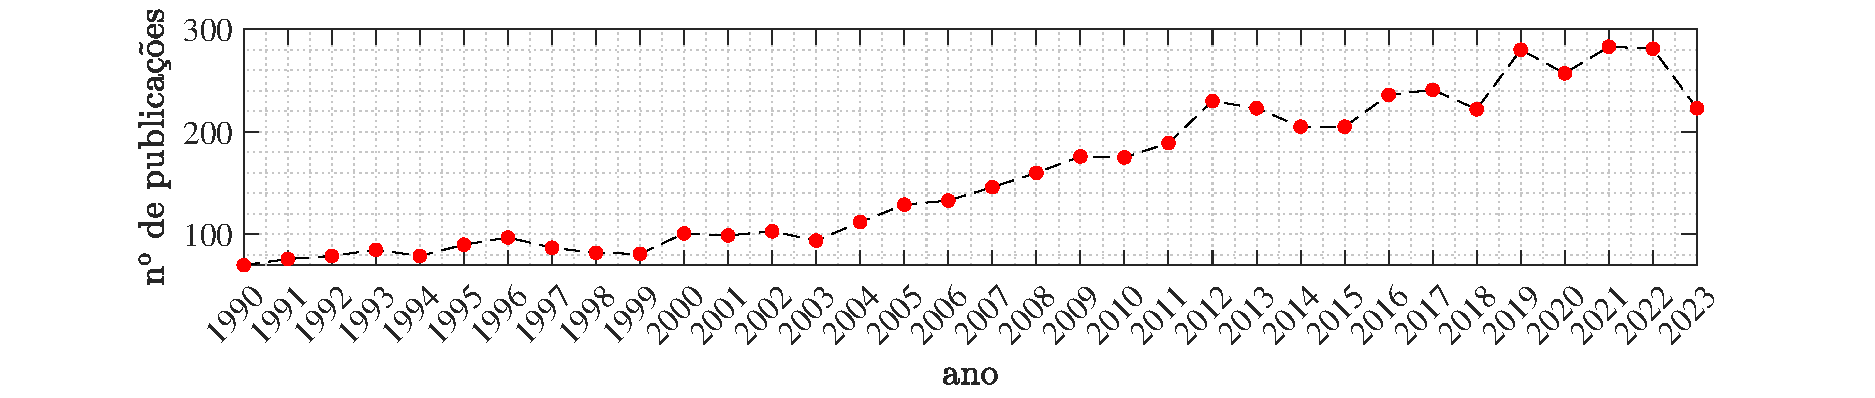
\includegraphics[scale=0.58,trim=20mm 0mm 0mm 0mm,clip=true]{figuras/wosblockoriented}
	\caption[Resultado da busca ``\textit{block-oriented models}'', ``\textit{Hammerstein models}'' e ``\textit{Wiener models}'' no \textit{Web of Science} em 18 de janeiro de 2024.]{Resultado de busca no \textit{Web of Science} em 18 de janeiro de 2024 para artigos com os termos ``\textit{block-oriented models}'', ``\textit{Hammerstein models}'' e ``\textit{Wiener models}'' presentes no título.}
	\label{fig:wos}
\end{figure}
%
\par 
Neste trabalho a dinâmica linear será representada em espaço de estados devido à sua harmonia com casos multivariáveis e ao número de ferramentas para projeto de controladores disponíveis para estes tipos de modelos~\citep{bai2010,borjas2012}. Embora as técnicas modernas de projeto de controle tenham evoluído com base em uma abordagem no espaço de estados, os métodos clássicos de identificação de sistemas foram desenvolvidos empregando a estrutura de entrada e saída que caracteriza as funções de transferência. Na década de 1990 que o conceito de estado foi popularizado na identificação de sistemas, desenvolvendo assim muitos métodos de subespaço baseados na teoria clássica estocástica de realização~\citep{verhaegen1992a,verhaegen1992b,van1994,katayama2005}.
\par 
Embora tenham ocorrido avanços relevantes nas últimas décadas, pesquisas que utilizam técnicas de identificação por subespaço para identificar não linearidades combinadas com modelos em espaço de estados são escassas, particularmente quando se trata de não linearidades fortes~\citep{aissaoui2016,noel2017}. Sendo assim, propõe-se como objeto de pesquisa desta dissertação a identificação de modelos de blocos interconectados por meio de técnicas de subespaços no cenário de não linearidades fortes. Tendo como horizonte a adequação do modelo em espaço de estados ao caso multivariável, os modelos de Hammerstein serão investigados, cujas curvas não lineares podem ser estáticas ou quase estáticas. Inicialmente, serão estudadas as formas de representação das curvas não lineares estáticas e quase estáticas com o intuito de modelar não linearidades fortes. O passo seguinte é aplicar essas técnicas junto aos métodos de subespaços, que no escopo deste trabalho será o \acs{MOESP}.




\section{Formulação Geral do Problema} \markright{\thesection ~~~ Formulação Geral do Problema}
\label{sec:intro_problema}
%
\par 
Os dois modelos clássicos de blocos interconectados consistem na associação em cascata de uma parcela dinâmica linear e outra estática não linear. A ordem relativa dos blocos define se a estrutura é de Hammerstein ou de Wiener, como pode ser observado de forma gráfica na Figura~\ref{fig:cap1modhamwin}.
%
\begin{figure}[h]
	\centering
	\begin{tabular}{c}
		a) \\
		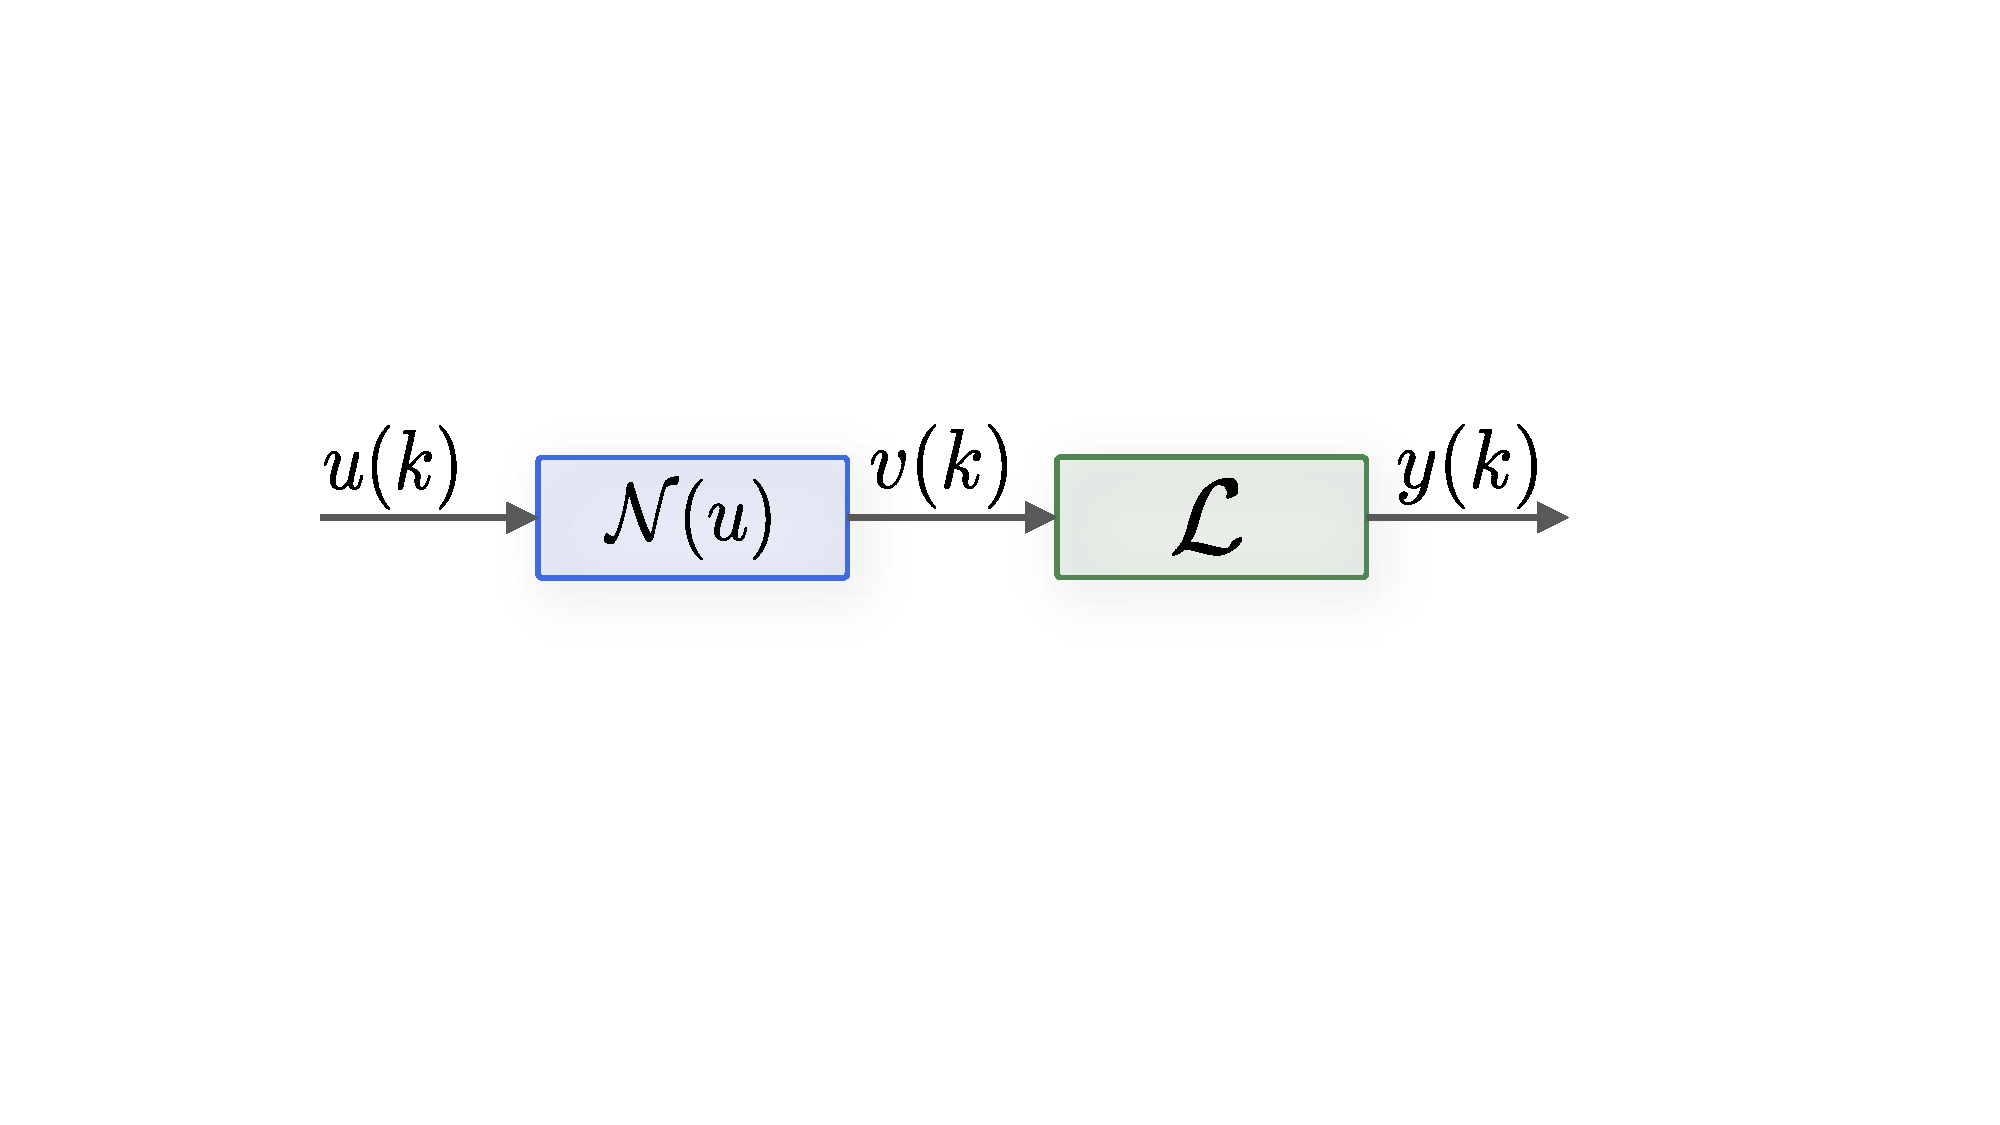
\includegraphics[scale=0.4,trim=0mm 80mm 8mm 65mm,clip=true]{figuras/ham_ger} \\
		b) \\
		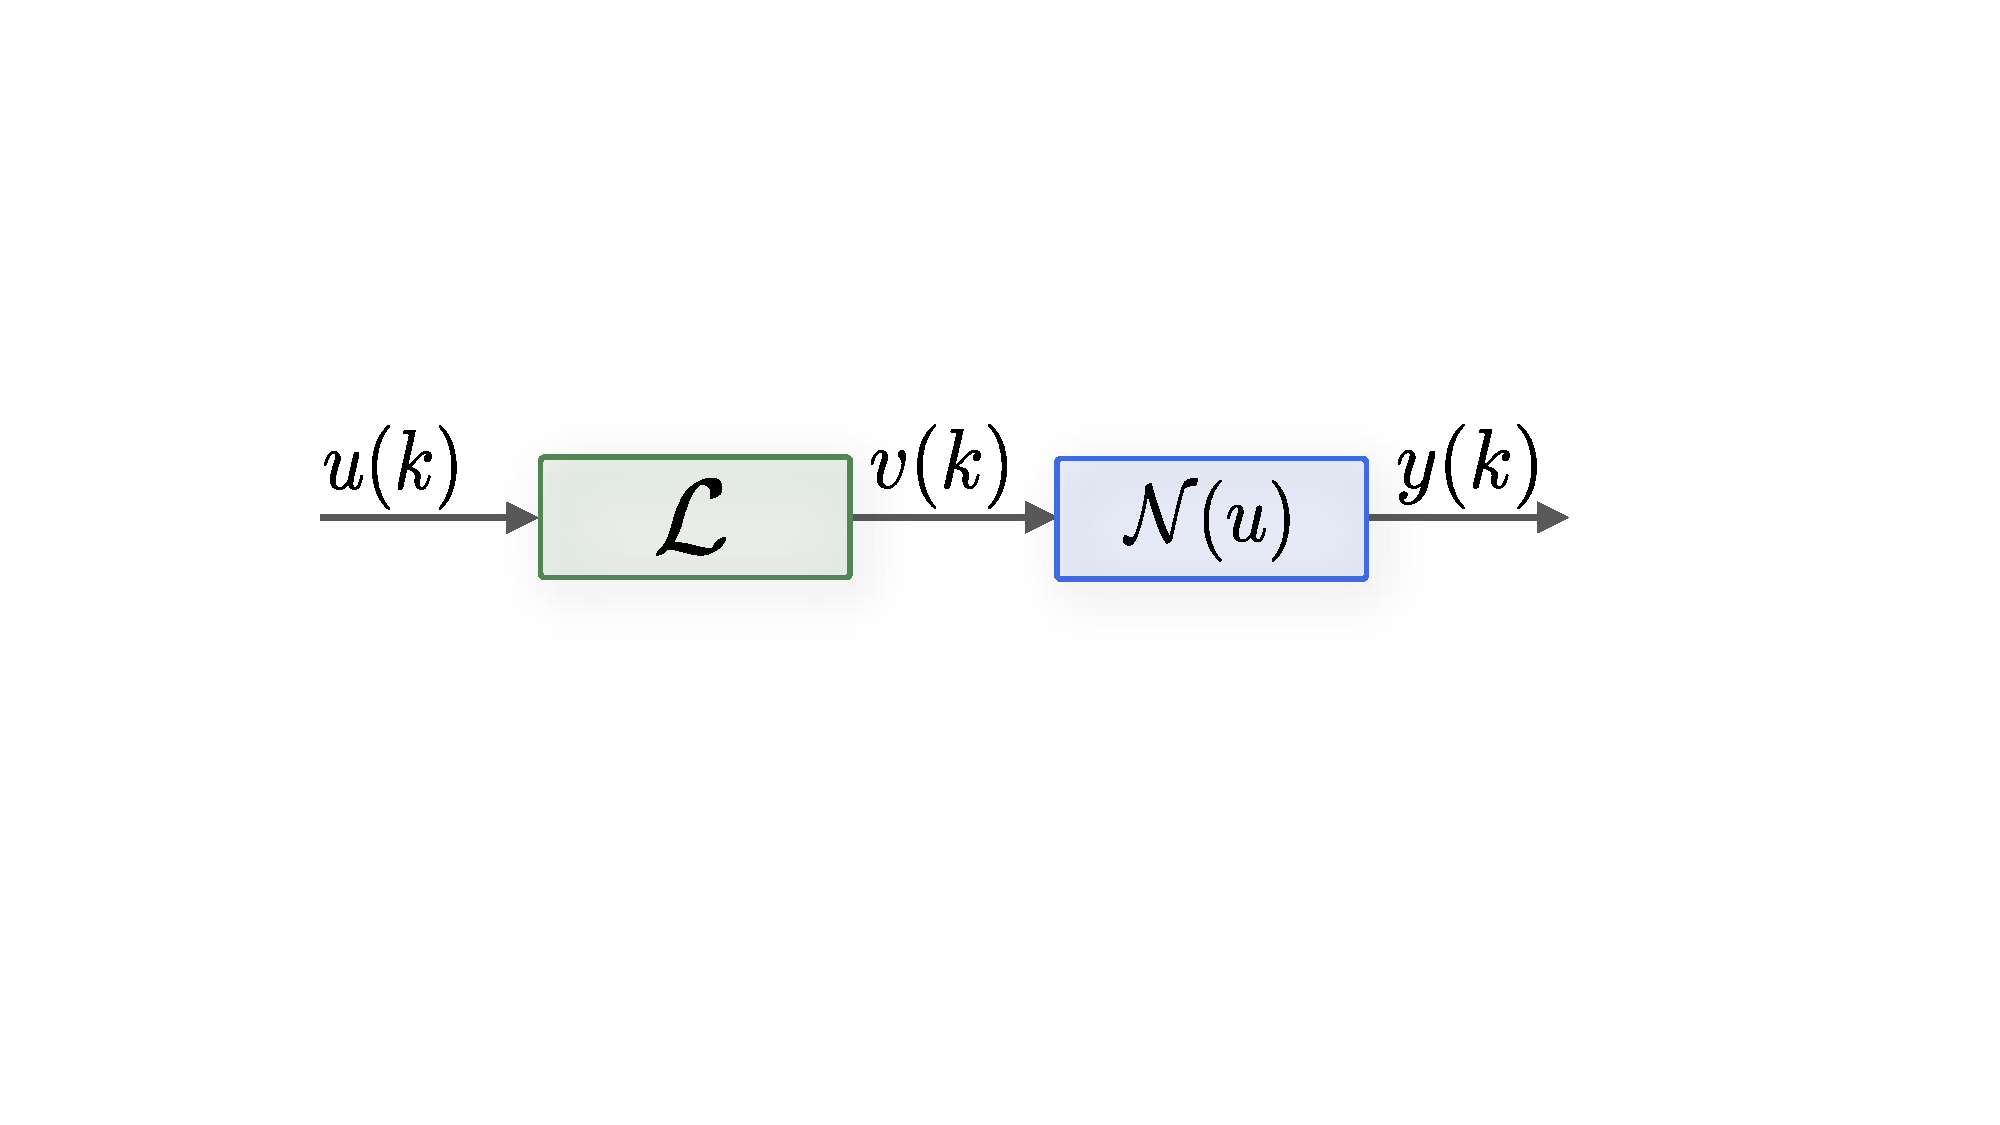
\includegraphics[scale=0.4,trim=0mm 80mm 8mm 65mm,clip=true]{figuras/wie_ger}
	\end{tabular}
	\caption[Estruturas clássicas dos modelos de blocos interconectados em malha aberta.]{Estruturas clássicas dos modelos de blocos interconectados em malha aberta com $p$ entradas $u(k)$, $\varrho$ sinais intermediários $v(k)$ e $m$ saídas $y(k)$. Em a) apresenta-se o modelo de Hammerstein composto por um subsistema não linear $\mathcal{N}$ seguido de um \acs{LIT} $\mathcal{L}$. Na parte b) do diagrama o modelo de Wiener composto pelos mesmos blocos em ordem invertida é apresentado.}
	\label{fig:cap1modhamwin}	
\end{figure}
%
\par 
Ambos blocos dos sistemas, de Hammerstein ou de Wiener, podem ser representados por modelos paramétricos ou não paramétricos. Exemplos amplamente conhecidos na literatura para representar sistemas \acs{LIT} são os modelos autorregressivos, em espaço de estados e a resposta em frequência~\citep{bai2010}. Por sua vez, a não linearidade pode ser retratada por variadas representações, sobretudo devido à especificidade do problema não linear. Alguns exemplos incluem funções polinomiais e sistemas \textit{fuzzy}. 
\par 
Considere a estrutura apresentada na Figura~\ref{fig:cap1modhamwin}~a) que configura o modelo de Hammerstein. Os sinais escritos no diagrama são: $u(k) \in \mathbb{R}^{ p }$, que porta os dados da entrada do sistema, $v(k) \in \mathbb{R}^{ \varrho }$, que representa os sinais intermediários e $y(k) \in \mathbb{R}^{ m }$, que informam acerca dos sinais medidos na saída do processo. 
\par 
Quanto aos subsistemas, o primeiro a aparecer, na forma de um retângulo azul, é o não linear que pode ser estático ou quase estático, monovariável ou multivariável, forte ou suave, representado pela notação $\mathcal{N}(u(k))$. Ou seja, é uma nomenclatura geral para uma função que represente a não linearidade. O fluxo de sinais intercorre conforme indicado pelas setas. Portanto, as amostras de entrada do processo $u(k)$ são mapeadas pela não linearidade $\mathcal{N}(u(k))$ produzindo o sinal intermediário $v(k)$. Esse sinal $v(k)$, em geral, não está disponível para medição. Note que $\mathcal{N}$ é uma transformação não linear que leva do espaço de dimensão $p$ da entrada para o espaço de dimensão $\varrho$ do sinal intermediário. 
\par 
Na formulação geral do problema apresentada nesta seção, a não linearidade permanecerá generalizada e sem representação definida, uma vez que ela será diferente para cada um dos cenários a serem detalhados no decorrer do texto, ou seja, não linearidade com e sem memória.
\par 
O segundo subsistema observado na Figura~\ref{fig:cap1modhamwin}~a), representado por $\mathcal{L}$ dentro do retângulo verde, é o modelo \acs{LIT}. Ele, por sua vez, é responsável por estabelecer uma relação dinâmica entre os dados intermediários e os dados de saída do processo. Neste trabalho o estudo será feito com base nos modelos em espaço de estados devido à sua harmonia com casos multivariáveis. Dito isso, a descrição matemática do modelo de Hammerstein é 
%
\begin{subequations}
	\begin{align}
		v(k) &= \mathcal{N}(u(k)),\\
		x(k+1) &= Ax(k) + Bv(k),\label{eq:cap1ee1}\\
		y(k) &= Cx(k) + Dv(k) + w(k),\label{eq:cap1ee2}
	\end{align}
	\label{eq:ee2cap1}
\end{subequations}
%
\hspace{-1.5mm}em que $u(k)$, $v(k)$ e $y(k)$ são os sinais de entrada, intermediário e de saída do processo, respectivamente. O vetor $x(k) \in \mathbb{R}^{ n }$ contém os $n$ estados do processo, $w(k) \in \mathbb{R}^{ m }$ é uma sequência de ruído branco de medição, estacionária e com média zero que contamina $y(k)$. $A \in \mathbb{R}^{ n\times n }$ é a matriz dinâmica do sistema, completamente caracterizada por seus autovalores. $B \in \mathbb{R}^{ n\times \varrho}$ é a matriz de entrada que representa a transformação linear pela qual os sinais intermediários influenciam o próximo estado. $C \in \mathbb{R}^{ m\times n }$ é a matriz de saída que descreve como o estado interno é transferido para o mundo exterior nas medições $y(k)$. E, por fim, a matriz $D \in \mathbb{R}^{ m\times \varrho}$ é denominada termo de transmissão direta por ser responsável por determinar a intensidade com que cada entrada afeta diretamente a saída.
\par 
É importante notar que os blocos do modelo podem não corresponder a componentes físicos do processo, uma vez que o sinal intermediário também é desconhecido e pode não existir. A inacessibilidade de tais medições, juntamente com as não linearidades do sistema, tornam a identificação dos modelos de blocos interconectados um desafio. 
\par
A dinâmica linear é descrita em espaço de estados pelas matrizes $A, \, B, \, C$ e $D$ e a função não linear por $\mathcal{N}$ que pode ser descrita por funções de base radial, polinômios, e sistemas \textit{fuzzy} no caso estático ou modelos de Bouc-Wen, Preisach ou \acs{P-I} no caso da histerese~\citep{noel2017}. Além disso, as seguintes suposições são estabelecidas acerca do processo e seus sinais.
\par
\begin{suposicao}
	O processo está disponível para realizar testes.
\end{suposicao}
\begin{suposicao}
	O processo a ser identificado é estável em malha aberta.
\end{suposicao}
\begin{suposicao}
	Os dados são coletados do processo em malha aberta.
	\label{sup:malha_aberta}
\end{suposicao}
\begin{suposicao}
	O sinal de entrada $u(k)$ é limitado em amplitude.
\end{suposicao}
\begin{suposicao}
	O sinal de ruído $w(k)$ é  um processo aleatório i.i.d de amplitude limitada.
\end{suposicao}
\begin{suposicao}
	O sinal intermediário ${v}(k)$ é inacessível, mas $u(k)$ e $y(k)$ são acessíveis.
\end{suposicao}
\begin{suposicao}
	A não linearidade $\mathcal{N}$ é forte.
\end{suposicao}

\par 
Desse modo, pode-se estabelecer o seguinte problema geral no contexto desta dissertação, cujo esquema é ilustrado na Figura~\ref{fig:cap1idconceito}.
\begin{problema}
	Obter estimativas da ordem $n$ do sistema, das matrizes $[A,~B,~C,~D]_{\mathcal{T}}$, em que $\mathcal{T}$ é uma transformação de similaridade desconhecida e dos parâmetros das funções não lineares $\mathcal{N}$ por meio dos dados de entrada e saída medidos do processo não linear em tempo discreto $\{u(k),y(k)\}$ de modo a reduzir o erro entre os sinais produzidos pela saída do modelo e do processo quando a entrada dos dois é idêntica.  
\end{problema}
%
\begin{figure}[h]
	\centering
	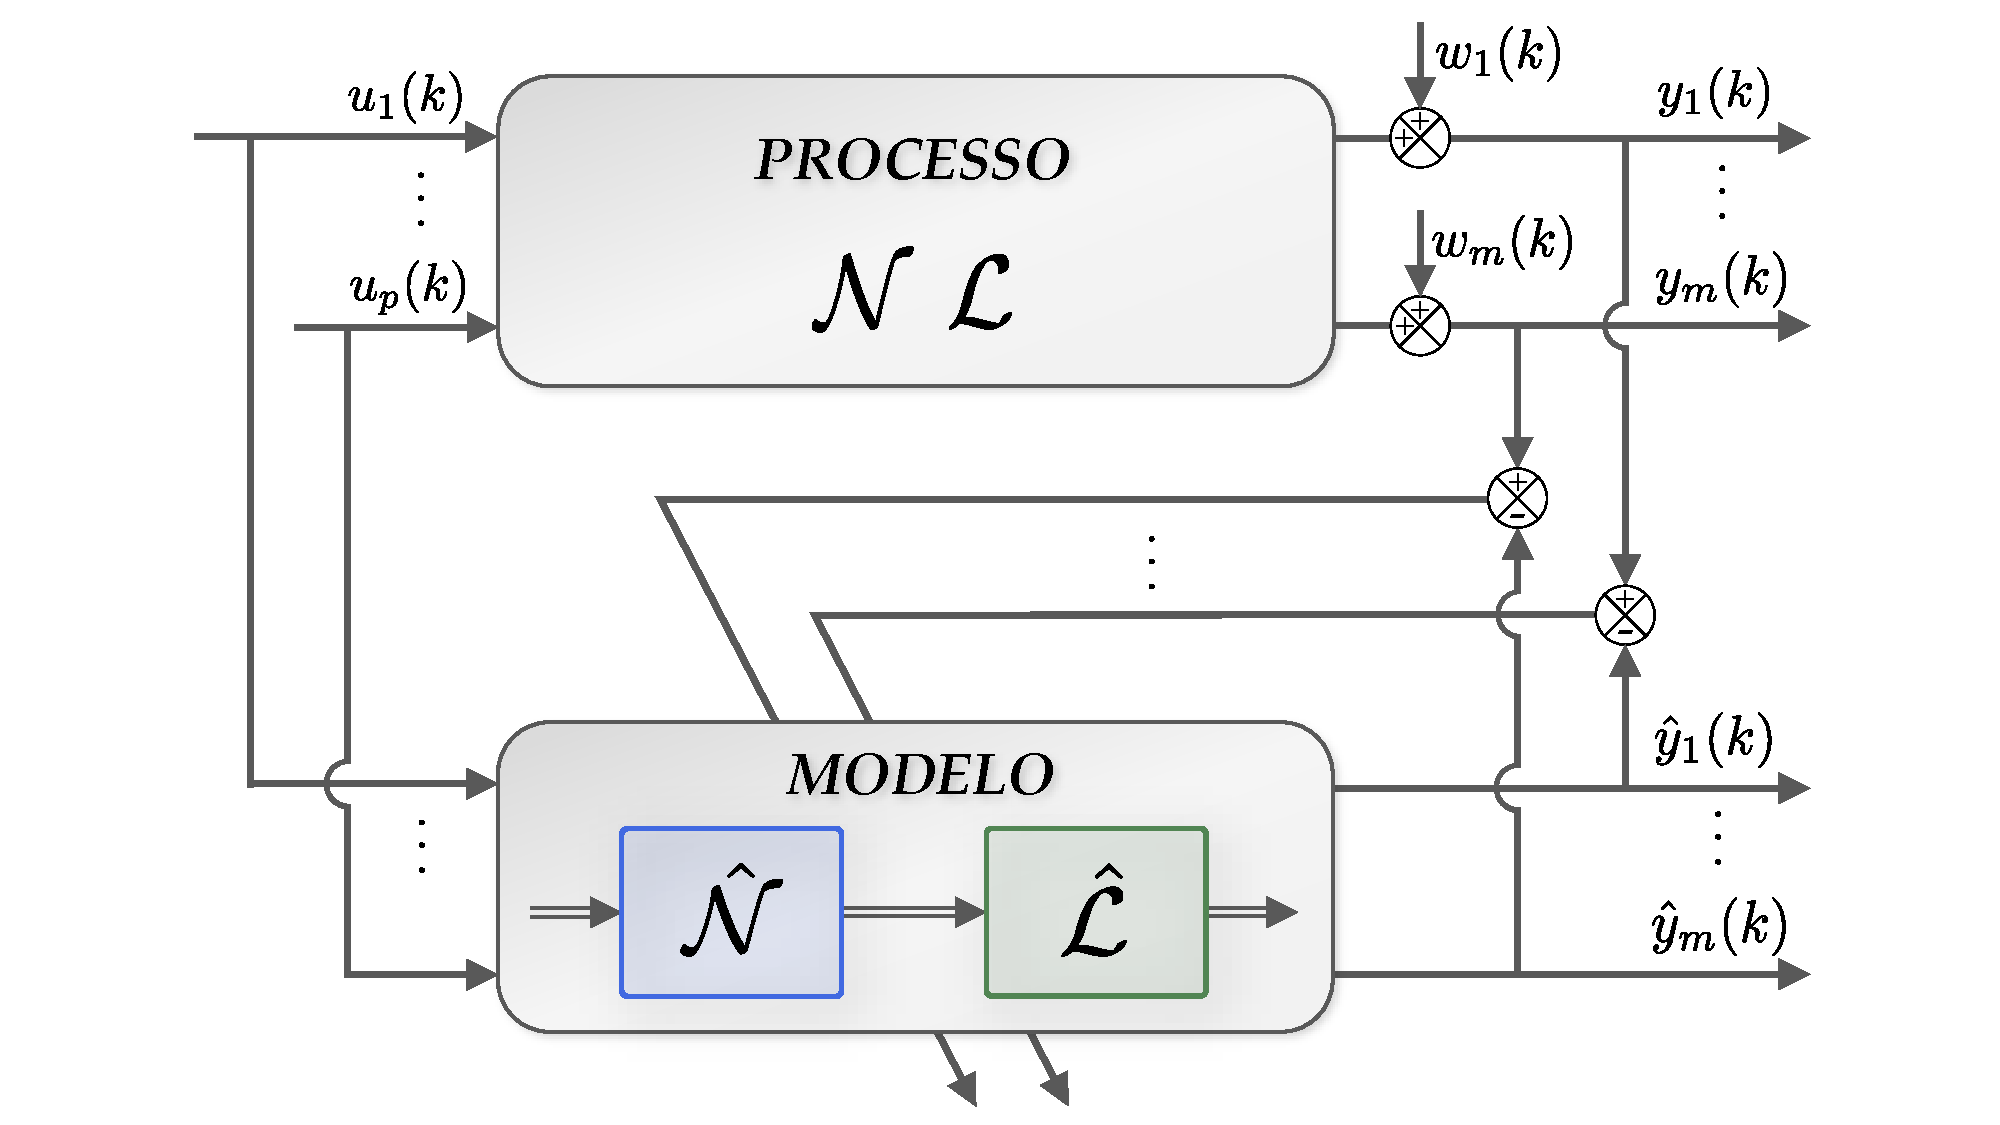
\includegraphics[width=0.9\linewidth]{figuras/cap1_idconceito}
	\caption[Esquema da maneira geral como a identificação de sistemas funciona.]{Esquema da maneira geral como a identificação de sistemas funciona. Os parâmetros do modelo são geralmente ajustados em função do erro entre a saída estimada pelo modelo e o saída do processo.}
	\label{fig:cap1idconceito}
\end{figure}
%

\section{Objetivos da Pesquisa} \markright{\thesection ~~~ Objetivos da Pesquisa}
\label{sec:intro_objetivo}


O objetivo geral desta dissertação é investigar metodologias de identificação de modelos de Hammerstein por métodos de subespaços a fim de caracterizar processos com não linearidades fortes. 

%\subsection{Objetivos específicos}
%\label{subsec:intro_objetivo}
Têm-se como objetivos específicos neste trabalho:
\begin{itemize}
	\item estudar as representações de não linearidades fortes na estrutura de blocos interconectados de Hammerstein contemplando não linearidades estáticas e quase estáticas;
	
	\item estudar os métodos de subespaços e os sinais de teste para identificar corretamente um modelo em espaço de estados linear na estrutura de Hammerstein \acs{MIMO} sem ter acesso ao sinal intermediário;
	
	\item propor um método de identificação para estimar uma rede \acs{NF} \acs{MIMO} que represente as curvas estáticas não lineares e um modelo em espaço de estados multivariável que exprima a dinâmica linear sem a necessidade de qualquer conhecimento prévio a respeito do processo;
	
	\item identificar um modelo \acs{GRDPI} \acs{MIMO} que descreva laços de histerese assimétricos e dependentes da taxa em conjunto com um modelo em espaço de estados multivariável;
	
	\item implementar exemplos numéricos que possam validar a possibilidade de aplicação dos métodos de identificação propostos em processos com não linearidades fortes multivariáveis.
\end{itemize}

\section{Estrutura da Dissertação} \markright{\thesection ~~~ Estrutura da Dissertação}
\label{sec:intro_estrutura}
%
\par
Esta dissertação está organizada em cinco capítulos, incluindo este, em que se motivou o estudo a partir de uma breve análise da literatura. Também neste primeiro capítulo foi apresentado o problema de pesquisa, bem como os objetivos a serem atingidos com o desenvolvimento do estudo.
%
\par
Para inteirar o leitor quanto aos assuntos tratados na dissertação, apresenta-se, no Capítulo~\ref{cap:rev}, a revisão de métodos e conceitos fundamentais que permeiam a identificação de modelos de blocos interconectados, especificamente, trata-se das representações de cada uma das parcelas linear e não linear que compõe os \acsp{MBI}.
%
\par
No Capítulo~\ref{cap:res1}, apresenta-se uma proposta de identificação de não linearidades estáticas fortes, como uma curva sinuosa com descontinuidades, empregando uma metodologia \acs{NF} junto com os métodos de  subespaços para identificação. A metodologia \acs{NF} proposta é capaz de identificar os parâmetros do modelo de Hammerstein cuja não linearidade seja representada por uma rede neural e a dinâmica linear em espaço de estados. Por fim apresentam-se alguns exemplos a fim de verificar a funcionalidade das metodologias.
%
\par
O Capítulo~\ref{cap:res2} é destinado a uma segunda proposta para identificação de não linearidades quase estáticas, a histerese. Nesta situação emprega-se um algoritmo de otimização amplamente conhecido, o de otimização por enxame de partículas (\acs{PSO}, do inglês \textit{Particle Swarm Optimization}), com algumas modificações para identificar os parâmetros da parcela não linear do modelo de Hammerstein. A parcela dinâmica linear é identificada separadamente por meio de um algoritmo de subespaços. Nesse capítulo também apresentam-se alguns exemplos para verificar as metodologias.
%
\par
Por fim, no Capítulo~\ref{cap:conc}, retoma-se a atenção às principais contribuições do trabalho e sugere-se perspectivas de temas para que sejam dadas continuidades a esta pesquisa. 
\clearpage



\clearpage
\thispagestyle{empty}
\cleardoublepage

%--------------------------------------------------------------------
%Capítulo 2 - Revisão Bibliográfica
%------------------------------------------------------------------------------
\chapter{Revisão sobre Identificação de Sistemas Não Lineares}
%
\label{cap:rev} \vspace{-1cm}  \vspace{1cm}
%
\section{Introdução} \markright{\thesection ~~~ Introdução}
%
\label{sec:rev_intro}
%
\par 
A identificação...
%
\section{Modelos de Blocos Interconectados} \markright{\thesection ~~~ Modelos de Blocos Interconectados}
%
\label{sec:rev_mbi}
%
\par
Os \acsp{MBI} são constituídos de dois subsistemas elementares que são os dinâmicos \acsp{LIT} e os elementos estáticos ou quase estáticos não lineares...

\section{Conclusão} \markright{\thesection ~~~ Conclusão}
\par 
Texto

%
\clearpage
%
\clearpage
\thispagestyle{empty}
\cleardoublepage

%--------------------------------------------------------------------
%Capítulo 3 - Análise de Dados
%-------------------------------------------------------------------------------
\chapter{Identificação de Não Linearidades Fortes Empregando a Metodologia \acs{NF}}
\label{cap:res1} \vspace{-1cm} \vspace{1cm}
%
\section{Introdução}  \markright{\thesection ~~~ Introdução}
%
\label{sec:res1_intro}
%
\par
No Capítulo~\ref{cap:rev}

\section{Exemplo Numérico} \markright{\thesection ~~~ Exemplo Numérico}
%
\label{sec:res1_exe}
%
\par
Nesta seção...


\section{Conclusão} \markright{\thesection ~~~ Conclusão}
%
\label{sec:conc_NF+MOESP}
%
Neste capítulo...

%
\clearpage
%






\clearpage
\thispagestyle{empty}
\cleardoublepage

%%--------------------------------------------------------------------
%%Capítulo 4 - Metodologias de Previsão
%-------------------------------------------------------------------------------
\chapter{Identificação de Histerese \acs{MIMO} Empregando \acs{MPSO} e Métodos de Subespaço}
\label{cap:res2} \vspace{-1cm} \vspace{1cm}
%
\section{Introdução}  \markright{\thesection ~~~ Introdução}
%
\label{sec:res2_intro}
%
\par
Uma particularidade...

\section{Modelo \acs{GRDPI} Multivariável} \markright{\thesection ~~~ Modelo \acs{GRDPI} Multivariável}
\label{sec:grdpimulti}
\par 
A parcela...
%
\section{Conclusão} \markright{\thesection ~~~ Conclusão}
\label{sec:conc}
%\vspace{-0.3cm}
Nesse capítulo...

%
\clearpage
%



\clearpage
\thispagestyle{empty}
\cleardoublepage
%
%%--------------------------------------------------------------------
%Capítulo 5 - Resultados Experimentais
%-------------------------------------------------------------------------------
\chapter{Exemplos Numéricos}
%
\label{cap:exem} 
%
\section{Identificação de não linearidades fortes usando modelos de Hammerstein} \markright{\thesection ~~~ Identificação de não linearidades fortes usando modelos de Hammerstein}
%
\label{sec:exem_ident}
%

%
\subsection{Associação das metodologias Neuro-Fuzzy e de subespaços}
%
\label{subsec:exem_NF+Subspace}
%

%
\subsection{Associação das metodologias MPSO e de subespaços} 
%
\label{subsec:exem_MPSO+Subspace}
%

%
\clearpage
%
\clearpage
\thispagestyle{empty}
\cleardoublepage

%--------------------------------------------------------------------
%Capítulo 5 - Conclusões
%-------------------------------------------------------------------------------
\chapter{Conclusões e Propostas para Trabalhos Futuros}
%
\label{cap:conc} \vspace{-1cm} \vspace{1cm}
%

\section{Considerações Finais} \markright{\thesection ~~~ Considerações Finais}
%
\label{sec:conc_resumo}
%
\par 
As pesquisas...
%
\section{Propostas de Trabalhos Futuros} \markright{\thesection ~~~ Propostas de Trabalhos Futuros}
%
\label{sec:conc_future}
%
Durante a condução dessa pesquisa foram observadas possibilidades de contribuições relacionadas ao tema em estudo. Ademais, com essas contribuições, surgiram perspectivas de extensões que podem ser implementadas em trabalhos futuros. Enumera-se a seguir pontos importantes para a continuidade deste trabalho. 
\begin{enumerate}
	\item Descrição...
\end{enumerate}


%
\clearpage
%
\clearpage
\thispagestyle{empty}
\cleardoublepage

%--------------------------------------------------------------------
%Bibliografia
%--------------------------------------------------------------------
%Definição de cabeçalhos

\bibliographystyle{apalike-brasil} %plainnat_mod
\bibliography{referencias}
\addcontentsline{toc}{chapter}{Bibliografia}
\clearpage
\thispagestyle{empty}
\cleardoublepage
%--------------------------------------------------------------------
% Apêndices
%\appendix\chapter{Título A}

%--------------------------------------------------------------------
\end{document}
